% !TeX root = ../main.tex
% Add the above to each chapter to make compiling the PDF easier in some editors.

\chapter{Background}\label{chapter:Background}
Since the main objective of this thesis is the development of a Blockchain-based system prototype for a decentralized index fund with an Ethereum-based index token, the background knowledge required is mainly from the Blockchain technology and the Ethereum ledger. As such, both Blockchain and Ethereum will be extensively reviewed in this chapter. A decently deep understanding of these topics will be greatly helpful with respect to designing and developing a secure and efficient DeFi application.

It should be noted that, this \textit{Background} chapter is by no means an exhaustive introduction of blockchain or Ethereum, but its purpose is rather to prepare a comprehensive foundation of the concepts relevant for the development of cryptographic tokens on Ethereum in the context of Decentralized Finance, which is the main topic of the thesis.

% \section{Asset Management Fundamentals}

% \subsection{Asset Management in Finance}

% Talks about the fundamentals of active and passive asset management

% \subsection{Passive Investment Funds}

% How they works?

% \subsubsection{Mutual Funds}

% what are the differences between Mutual vs. Index vs. Exchange Traded Funds?

% Dividend funds

% Real-world examples?

% \subsubsection{Index Funds}

% \subsubsection{Exchange Traded Funds}



% #################################################################################
\section{Blockchain Fundamentals} \label{sec:blockchainfund}
The idea of Blockchain was initially introduced in 1991 by Stuart Haber and W. Scott Stornetta in their paper on \textit{How to Time-stamp Digital Documents} \cite{haber1990time} and the followup paper \textit{Improving the Efficiency and Reliability of Digital Time-Stamping} in 1992 \cite{bayer1993improving}, but the concept has only gained significant attention and become popular since the publication of the Bitcoin's white paper by the pseudonymous author or authors named Satoshi Nakamoto in 2008 \cite{satoshi2008peer}. Since then, the prospects of this innovative technology and other types of Distributed Ledger Technology have been widely investigated for potential applications in academy as well as in many industries, especially in the financial sector \cite{swan2017anticipating}. The most common application of Blockchain is in the financial context, in which Blockchain enables building global transactional systems for transferring digital assets in a direct peer-to-peer fashion without the need for a third-party intermediary such as a central bank \cite{swan2015blockchain}. This eliminates many types of costs related to the development and maintenance of such centralized electronic funds transfer systems, and consequently, reduces the transaction costs. In order to allow financial transactions to be performed in a decentralized manner, blockchain relies on a number of cryptographic constructions to solve the trust issue between the sender and the recipient of the funds when there is no trusted third-party to ensure non-reversible payments. Such benefits and applications from blockchain are enabled by a clever combination of cryptography with a consensus algorithm and a handful of efficient data structures. Therefore, it is essential to have a good understanding of the primitives and constituting components of blockchain before developing a system based on it.

% its key characteristics and
%  Note that, the technical details in this \textit{Background} section will refer to the Bitcoin's white paper \cite{satoshi2008peer}, therefore, the citations to that white paper will be omitted in the rest of this section to enhance the readability. 




\subsection{Cryptographic Hash Functions} \label{subsec:hashfunc}

Physical currencies normally contain many security measures to make the process of counterfeiting harder and more costly. In quite the same manner, cryptocurrencies, as the name implies, rely on cryptography to add countermeasures against forgery and fraudulence. The two most important cryptographic building blocks that provide security mechanisms to cryptocurrencies and allow them to be operational in practice are \textit{hashes} and \textit{digital signatures} \cite{narayanan2016bitcoin}, of which hashes are the cryptographic primitive at the core of blockchain and play an important role to the structure as well as the validity of the chain. In fact, a hash is the output of a \textit{hash function} and is also commonly called hash values, hash codes or \textit{digests} \cite{enwiki:1029031919}. In the famous \textit{"Handbook of Applied Cryptography"} by Menezes et al. \cite{menezes1997handbook}, a \textit{generic} hash function is defined as follows.

\begin{definition}[\textbf{\textit{Hash function}}]\label{hashfunc_def}
A \textit{hash function} is a function $h$ which has, as a minimum, the following two properties:
\begin{itemize}
    \item \textbf{Compression} --- \textit{$h$ maps an input $x$ of arbitrary finite bit length, to an output $h(x)$ of fixed bit length $n$.}
    \item \textbf{Ease of Computation} --- \textit{Given $h$ and an input $x$, the output $h(x)$ is easy to compute.}
\end{itemize}
\end{definition}

Definition \ref{hashfunc_def} introduces the two most common properties for a function to be called a hash function. The compression property can be expressed mathematically as $h: \{0,1\}^{*} \rightarrow \{0,1\}^n$, which means $h$ \textit{compresses} the input of any size in binary representation to an output that always has a fixed size of $n$ bits. The second property simply states that $h$ should be able to compute the output $h(x)$ in a reasonable amount of time, or more technically, the output of an $m$-bit input should be computed in $O(m)$ time and space.

\subsubsection{Cryptographic Properties of Hash Functions}

Due to the significant role of hashes to the security of blockchain, additional properties are desirable to make a hash function to be \textit{cryptographically secure}. For this, a hash function is required to have the following properties in addition to the two above: \textit{preimage resistance}, \textit{2nd-preimage resistance} and \textit{collision resistance}. These properties are defined in \cite{menezes1997handbook} for a hash function $h$ as follows.

\begin{itemize}
    \item \textbf{Preimage Resistance} --- \textit{For essentially all pre-specified outputs $y$, it is computationally infeasible to find an input $x$ such that $h(x) = y$.}
    \item \textbf{2nd-Preimage Resistance} --- \textit{Given input $x$, it is computationally infeasible to find any second input $x'$ with $x' \neq x$ such that $x'$ hashes to the same output as $x$, or in other words, such that $h(x') = h(x)$.}
    \item \textbf{Collision Resistance} --- \textit{It is computationally infeasible to find any two distinct inputs $x$ and $x'$ which hash to the same output, i.e., such that $h(x) = h(x')$.} 
\end{itemize}

The term "computationally infeasible" used in the three properties above can be understood as referring to a "hard instance of an NP-Hard problem of sufficient size", where a \textit{hard instance} means trying all possible solutions is the only single approach to solve the problem and \textit{sufficient size} implies a size so large that it would take a classical computer literally not less than the age of the universe to solve the problem \cite{henderson1976cryptography}.  
Regarding the meaning of the properties themselves, the \textit{preimage resistance property} suggests that the inverse function $h^{-1}$ should not exist, and therefore, the only way to find the input from the known output is to brute-force a large input space, which can be indefinite in size. Next, the property of \textit{2nd-preimage resistance} means that there exists no efficient approach other than exhaustively searching through every single possible input to find a valid input $x'$ different from $x$ but hashes to the same output as $x$. In contrast to the 2nd-preimage resistance property, in which an input $x$ is \textit{given} and the problem instance is to find another input $x'$, the \textit{collision resistance property} allows that both distinct inputs $x$ and $x'$ can be freely chosen but such pair that have the same hash value  should not be computationally feasible to find. The term "collision" in the context of hash function indicates the situation, in which two different inputs hash to the same digest. As per the compression property presented in Definition \ref{hashfunc_def}, it follows that hash collisions are unavoidable and they always exist for any hash function. This is due to the fact that the input space of a hash function is indefinitely large, while the output space is finite and the \textit{pigeonhole principle} \cite{herstein1969topics} applies. Therefore, the collision resistance property does accept that collisions exist, but it requires that a classical computer needs an astronomically long time to find such collisions. To give a concrete example, consider the size of a hash value is $256$ bits, which means the output space contains $2^{256}$ possible values. Now, if $2^{256} + 1$ distinct inputs are hashed, it is guaranteed that at least one collision will occur. In fact, due to the \textit{birthday paradox} \cite{abramson1970more}, a collision can be found by only testing through approximately a square root of that number, which is about $2^{128}$ digests. However, if a modern computer can produce $10$ millions hashes per second, it would need roughly $10^{31}$ seconds to produce $2^{128}$ hash values and that is equivalent to more than $10^{23}$ years. For comparison, the age of the universe has been recently confirmed with $13.8 \times 10^9$ years \cite{aghanim2020planck}. Certainly, a collision can occur earlier before all $2^{128}$ hash values are exhaustively explored, but that should be purely random and the probability for that is also infinitesimally small.

As defined in \cite{menezes1997handbook}, when a hash function, addition to the inherent compression and ease of computation properties, has the properties of preimage resistance as well as 2nd preimage resistance, it is called a \textit{one-way hash function} and when it additionally has the resistance property, therefore, is characterized by all the five properties introduced so far, that hash function is defined as \textit{collision resistant hash function}. The term "one-way" indicates that the reversed direction to find the input from a given hash output is almost impossible.

\subsubsection{Useful Properties of Hash Functions for Cryptocurrencies}

Ultimately, the main purpose of hashing in blockchain is to detect data modification and ensure data integrity. Therefore, it is required that the employed hash function should be a \textit{collision resistance hash function} to fulfill those security requirements. Moreover, to be practically employable for cryptocurrencies, Narayanan et al. \cite{narayanan2016bitcoin} suggest two more properties for a hash function as follows.

\begin{itemize}
    \item \textbf{Hiding} --- \textit{Given the hash output $h(r \parallel x) = y$, where $r$ is a secret value chosen randomly from a probability distribution that has high min‐entropy, then it is infeasible to find the input $x$.} (Note that $\parallel$ is the concatenation symbol)
    \item \textbf{Puzzle Friendliness} --- \textit{For every possible hash output $y$ with length of $m$ bits, if $r$ is chosen from a distribution with high min‐entropy, then it is infeasible to find $x$ such that the hashing $h(r \parallel x) = y$ can run in time significantly less than $2^m$.}
\end{itemize}

A more comprehensive explanation of entropy can be found in the primer by Rioul \cite{rioul2018primer}. In a nutshell, \textit{min-entropy} is a notion used in information-theory to quantify the unpredictability of an outcome set. If a probability distribution has high min-entropy, that the distribution is then very spread out, or in other words, the underlying random variable is highly unpredictable. Consequently, if $r$ is sampled from such a distribution, then every value from the distribution is equally likely to be sampled, which makes the auxiliary part $r$ of the input impossible to be guessed given that the probability space is large enough. The \textit{hiding property} is useful when the input space of a hash function is rather small, and thus, the main input $x$ is trivial to be found. By concatenating an auxiliary value from a larger space, e.g, with a size of $2^{256}$, the input is no longer $x$ but $(r \parallel x)$, which is in a significantly larger input space. Since $r$ is very difficult to be guessed and should be longer than $x$ in bit size, along with $h$ being a one-way hash function, the only approach to find the the concatenated input $(r \parallel x)$ is to brute-force through the unified space of $r$ and $x$, which is, as discussed earlier, not computationally feasible if the space of $r$ is sufficiently large, for instance, $r \in \{0,1\}^{256}$. As a result, the \textit{hiding property} is a necessary security requirement in case the original input $x$ is predictable. This property finds its application in the so-called \textit{commitment scheme}, which is employed in blockchain for the block mining process.

On the other hand, the purpose of the \textit{puzzle friendliness property} is to guard against pre-computation of the solution for a mathematical problem called \textit{search puzzle}, for which the task is to search in a large space for a solution satisfying certain criteria. For example, if the problem is to search for the input part $x$ whose concatenation with a random value $r$ hashes to an output $y$ in a set $Y$. This problem instance is exactly what is applied in blockchain for mining new blocks, where $x$ is called the \textit{nonce} and $r$ is in fact the remaining part of a block. Intuitively, if some particular value $r$ is likely than others, then one can cheat by computing the solutions to the puzzle in advance using those likely values of $r$. Therefore, the \textit{puzzle friendliness property} ensures there are no shortcuts to solve a search puzzle rather than exhaustively examining every possible values in the space of $x$ and that will run in $O(2^m)$ since in the worst case, all $2^m$ hashes in the output space will be generated for the search.

In this section, seven properties of hash functions have been introduced. By definition, a general hash function has the compression and ease of computation properties. To be a \textit{cryptographic} hash function, a hash function has to additionally hold three more properties, which are preimage resistance, 2nd preimage resistance and collision resistance. For cryptocurrencies, a hash function is considered to be practically applicable if it is further characterized by the hiding and puzzle friendliness properties. In practice, there are various implementations of hash functions that satisfy all of those seven properties. For instance, SHA-256 is a well-known hash function employed in the Bitcoin's blockchain, while Ethereum applies SHA3-256 for its blockchain. It is worth noting that the properties discussed in this section are by no means an exhaustive list to secure a blockchain against all types of attack through its hash function. For instance, while \textit{preimage attack} and \textit{collision attack} can be prevented, the set of SHA-2 hash functions, of which the hash function SHA-256 used in Bitcoin is a member, still suffers from \textit{length extension attack} \cite{duong2009flickr}. Basically, different blockchain applications have different security requirements regarding hash function properties and there is no universal list of properties that a hash function must have to be completely secure. Nonetheless, the seven properties discussed in this section happen to be the standard ones that characterize the most commonly used hash functions in real-world blockchain applications, at least in the currently largest blockchains such as Bitcoin and Ethereum.  


% \subsection{Asymmetric Cryptography}

% \subsection{Digital Signatures}


\subsection{Data Structures} \label{subsec:datastructure}

The definition of hash functions along with their desirable properties presented previously form the foundation for the data structures implemented in blockchain. First of all, hash functions are employed to build the most primitive data structure of blockchain, the so-called \textit{hash pointer}. Then, based on hash pointers, a list structure called \textit{block chain} and a tree structure known as \textit{Merkle tree} are constructed and they constitute the two most fundamental building blocks of blockchain. These three data structures will be the main subjects for this section. 

\subsubsection{Hash Pointers} \label{subsubsec:hashpointer}

Being the most primitive data structure of blockchain, the concept hash pointer is quite straightforward: a hash pointer is basically a pointer to the location of certain information, in addition, it also stores the cryptographic hash of that information \cite{narayanan2016bitcoin}. In order words, a hash pointer still resembles a regular pointer, in which it is a data structure that does not store the information itself, but a reference to the actual information. Furthermore, a hash pointer also provides the ability to verify whether the information has been tampered with since the time it has been recorded. This \textit{tamper-evident} ability is enabled due to the fact that the cryptographic hash of that information is also stored in the hash pointer and the collision resistance property of the underlying hash function ensures that if the information is modified, then it will hash to a value different from the one stored in the hash point. As a result, the modification can be detected by comparing the two hash values.

In general, a hash pointer can be used to build any data structures that are commonly built with regular pointers as long as the data structure is \textit{acyclic} \cite{narayanan2016bitcoin}. Among others, list and tree data structures are the most common ones that utilize pointers for their construction and operations. As will be discussed in sections \ref{sec_chain_of_blocks} and \ref{sec_merkle_tree}, one can see that hash pointer indeed constitutes a linked list and a binary data structures, which provide blockchain many useful security features.

To summarize, a hash pointer consists of two parts: a location of the information and a digest of the information. In the context of blockchain, however, the location part is omitted and only the digest part is relevant since information can always be retrieved by querying other participants in the blockchain network. For this reason, a hash pointer in blockchain is only a fixed-length string of a hash value that can be used for the validation of data such as blocks and transactions. Since the term "hash pointer" in this thesis is always referred to in the context of blockchain, it will loosely be used to indicate the hash of some data as a means of data integrity validation throughout the thesis although this meaning partially deviates from the original definition.

\subsubsection{Chain of Blocks}\label{sec_chain_of_blocks}

Although being an innovative technology underpinning many transactional systems on a global scale such as Bitcoin and Ethereum, the core structure of blockchain is rather simple: blockchain is simply a specific type of database that manages a constantly growing set of data blocks being chained together in a chronological order by hash pointers. With respect to a certain block, the block preceding it is called the \textit{parent} block and the one succeeding it is its child block. Therefore, a blockchain is in fact a chain of data blocks resembling the familiar \textit{linked list} data structure with list elements being blocks. However, unlike a common linked list, in which list elements are linked by regular pointers, each block in a blockchain links to the immediately preceding block by a hash pointer.

By storing the hash pointer to its parent in the block header containing metadata, each block contains tamper-evident information of its parent with the only exception being the very first block called the \textit{genesis block}, which does not have hash pointer to any block since there exist no blocks before it. As a result, the integrity of a block can be verified by comparing its hash value with the one stored in the header of the child block. In case the block in question is the latest block in the chain, its cryptographic hash is then stored separately in the \textit{head} of the chain, which is a hash pointer that always points to the newest block of the chain. When there is a need to store new data items in the chain, an empty new block is created and the set of data items is included into this block. Then, this new block adds to its header the hash value of the most recent block in the current chain and the head of the chain is changed to point to this new block. After that, the appendage of a new block to the chain is completed. In this manner, a tamper-evident chain of blocks with arbitrary length can be constructed and the data can no longer be changed once it is stored in the chain. If a block $b$ in the chain is modified, then the inconsistency between the hash value of the modified block $b$ and the one in the metadata of block $b+1$ will be detected during the chain validation, which will render the chain to be invalid. Of course, an adversary can as well modify all the blocks starting from block $b+1$ to the most recent block in order to conceal the modification, however, the adversary will fail at the head of the chain if the head is protected against malicious manipulation. As such, the integrity of the entire chain can be ensured by storing only a single hash pointer. 

\subsubsection{Merkle Trees}\label{sec_merkle_tree}

While a linked list with hash pointer discussed in section \ref{sec_chain_of_blocks} is practical to ensure the integrity of all data, it is however not an efficient data structure for validating data inclusion since sequential traversal through the list is required to look for the data in question. As a result, the space and time complexity for such operations on a \textit{list} data structure is $O(n)$ with $n$ being the number of data. To allow for efficient validation of transactional data, blockchain employs a hash-pointer-based \textit{tree} data structure called \textit{Merkle Tree} \cite{merkle1982method, merkle1987digital}, which is basically a binary tree and commonly used as an efficient and secure approach to verify the content in a large body of data. Consequently, this reduces the complexity of the integrity validation down to $O(log(n))$ in time and space as there is no need to acquire the entire tree for validation, but only the nodes along a particular path are required. With respect to the structure, the most obvious difference between a Merkle tree and a regular binary tree is the use of hash pointers in place of regular pointers to the children nodes in a the next lower level. Each leaf node at the lowest level of a Merkle tree is essentially a cryptographic hash of an actual piece of data and except for the root node, a node in level $h$ is always paired with the next node in the same level such that the concatenation of their individual hash values serves as the input to generate the hash value for their common parent node in level $h-1$. For this reason, Merkle trees always require an even number of leaf nodes and in case the number of data records is an odd number, the last leaf node will be duplicated once to achieve an even number of left nodes. In this manner, a Merkle tree is constructed in the bottom-up fashion from the leaf nodes up to the root node at level $0$. 

For every path from the root node to each of the leaf node, there is a chain of hash pointers resembling the way how blocks in blockchain are linked together using hash pointers as described in section \ref{sec_chain_of_blocks}. Therefore, this provides same benefit of tamper-evident validation by just storing a single hash pointer at the head of the chain or in this case, storing only the hash value of the root node instead of the entire tree although the tree must be constructed first to obtain the root hash. On the other hand, the validation run-time is much faster with Merkle tree than with the linked list structure and also, the space required is significantly less. 
In fact, there are two types of validation that relies on Merkle tree in blockchain, they are \textit{proof of membership} and \textit{proof of non-membership} \cite{narayanan2016bitcoin} and can be described as follows.

\begin{description}
	\item[Proof of Membership] --- Given a particular data item and the root hash of a Merkle tree, one can prove that this data item is in fact part of the Merkle tree. To this end, the validating party needs the data item itself as well as all the data items on the path from the data item in question to the Merkle root. Then, the validation can be performed by hashing and constructing the path from that data item to the root. If the final hash value resulted from the validation matches the root hash stored by the validating party, then they can confirm that that data item has been used to produce the Merkle root and was not tampered with.	In blockchain, proof of membership is used extensively by the users to verify if a certain transaction has been mined in a block without retrieving the whole transaction set of that block. This is especially useful for \textit{Simplified Payment Verification Clients}, or SPV Clients for short, \cite{satoshi2008peer} as they have limited resources for the validation process.
	\item[Proof of Non-membership] --- Given a certain data item and the root hash of a \textit{sorted} Merkle tree, it is possible to show that the data item is not included in the Merkle tree. As the Merkle tree has its leaf nodes sorted in a specific order, one can simply perform two proofs of membership: each for the item right before and the one right after the data item in question. If the preceding and the succeeding data items happen to be consecutive in the specified order, then the item in question is definitely not part of the Merkle tree. Ultimately, the proof of non-membership is not different from proof of membership with respect to the execution.  
\end{description}

Through the explanation of proof of membership and non-membership, the benefit of Merkle tree over hash-pointer-based list is obvious since it is not necessary to have the complete data set in place, but only the data items on the relevant path to the root should be fetched at a time and the integrity of the path can be immediately verified. This considerably reduces the amount of memory and disk space required for the validation of only some certain items. Specifically, the space required is only of logarithmic magnitude to the number of data items since the number of nodes on a path from a leaf node to the root of a \textit{full} binary tree is equal to the height of tree, which is equivalent to $O(log(n))$ nodes with $n$ being the total number of nodes in the tree \cite{knuth1998vol3}. It should be noted that the number of leaf nodes in a full binary tree is $\lceil \frac{n}{2} \rceil$, therefore, the space complexity is still $O(log(n))$ if $n$ is the total number of data items. Since each node along the path will be hashed once to compute the root hash, the time complexity is therefore also $O(log(n))$. An additional benefit related to the improved space complexity compared to the linked list structure is that the amount of data transmitted across the network for the validation is much less, which is obviously beneficial for blockchain network.

\subsection{Basic Block Structure}

Based on the data structures introduced in section \ref{subsec:datastructure}, the structure of blocks can now be discussed in more detail in this section. In practice, different blockchain ledgers have slightly different specifications for their blocks depending on their application and the purpose. For example, Ethereum adds more complexity to the block structure compared to Blockchain to support more features such as smart contracts \cite{wood2014ethereum}. Although the Ethereum blockchain is more relevant for the purpose of our work, the structure of Bitcoin block in fact serves as the basis for that of Ethereum and is sufficient as a foundation for other discussions in the rest of this paper. Therefore, we will explore the structure of Bitcoin block and consider it as a general standard for our discussions involving block configuration, while the nuances of Ethereum block will be addressed specifically where necessary.


In general, a block is composed of two main parts: a \textit{block header} containing a set of metadata fields and a \textit{block body} consisting of multiple transactions. In Bitcoin, the average size of a transaction is about 250 bytes and there are normally more than 500 transactions included in a block, therefore, the block body is the part that is responsible for most of the block size with more than 1,500 times larger than the block header size. However, the header contains many critical information for the inner working of blockchain regarding the core structure of blockchain, cryptographic validation and consensus mechanism.

Except for the \textit{Version} field that holds the version number of the blockchain as a software product for tasks such as software upgrades and version control, the rest of the header fields are the ones crucial for the nuts and bolts of blockchain. First, the \textit{Previous Block Hash} is the SHA-256 hash pointer to the parent block and binds the current block to its parent, therefore, forming the core structure of blockchain as discussed in section \ref{sec_chain_of_blocks}. Next, the \textit{Merkle Root} field is another 32-byte hash value that represents the Merkle root for efficiently validating the transactions carried in the block body as explained in section \ref{sec_merkle_tree}. At this point, one can see that the integrity of a block is ensured by the \textit{Previous Block Hash} field, while the integrity of a transaction is secured by the \textit{Merkle Root} field of a block. As a result, every single transaction or data item in the entire blockchain is guaranteed to be tamper-evident by the combination of the two hash-pointer-based data structures that entail a linked-list and a binary tree. 
Finally, the \textit{Timestamp}, \textit{Difficulty Target} and \textit{Nonce} fields assemble a set of metadata involving the consensus protocol and Proof-of-Work mechanism that will be explored in section \label{subsubsec:pow}. 


\subsection{Decentralization and Consensus Protocol}

Decentralization is one of the most important characteristics of blockchain. It provides cryptocurrencies the main benefit over traditional currencies to be operational without the need of an intermediate authority such as a bank for executing transactions. In the context of network protocol, the term "decentralization" in fact refers to a network model, in which there are no centralized components that perform all the inner workings of the system such as mainframes or servers, but rather every machine or node in the system is equal and collectively share the network services to one another without forming any sort of hierarchy. As such, there is no concept of client-server in such network model and the model is often called \textit{peer-to-peer network} with every participant is called a \textit{peer} \cite{fox2001peer}. In practice, there is a wide range of well-known realizations of the peer-to-peer model such as Napster, Gnutella, Skype, BitTorrent and especially many instances of public blockchain ledges such as Bitcoin and Ethereum.


In fact, a public blockchain network is typically a peer-to-peer network with every node storing a full record of data in their local blockchain since the inception of the chain. This enables not only inherent data replication in the network, but also secured data validation and reliable data synchronization through some consensus protocol.Without relying on a certain centralized entity storing the data of the system, blockchain with its inherent data replication does not create \textit{single point of failure}, which is a potential risk that can render the whole system unavailable for many reasons such as cyber attacks, natural disasters or being shut down by authorities as in the case of Napster \cite{stern2000napster}. Furthermore, unilateral data manipulation and other types of intervention such as censorship from a minority of nodes have no effect on the final state of the chain once the network has achieved consensus on a legitimate state. For instance, a small number of nodes can arbitrarily modify the data in a certain block of their local blockchain for their benefits and create therefore a new sequence of hashes from that block to the head of the chain, but the modification will not be accepted by the rest of the network since the honest nodes still have the original version of the chain and they together comprise the majority of the network. In addition, no costs for developing the system and maintaining servers are incurred even if the system reaches the global scale.

Obviously, the riddance of centralized components in the system provides many benefits for the network as long as the network participants can reliably reach consensus on the shared data to ensure consistency and guard against malicious behaviors.
That being said, a reliable and secure consensus mechanism in distributed environment is actually a hard problem that exposes many impossibility results due to a variety of reasons such as network partitions, communication latency, lack of global time, adversarial behaviors and so on \cite{narayanan2016bitcoin}. As far as problem of distributed consensus is concerned, there is the classic \textit{Byzantine Generals Problem} from Lamport et al. \cite{lamport1982byzantine} showing that the number of honest nodes must occupy at least $2/3$ (two third) of the total number of nodes in the network in order to for the network to achieve consensus reliably. In open peer-to-peer systems, however, due to the fact that nodes join and leave the network frequently in addition to the non-deterministic number of malicious nodes, it is virtually impossible to guarantee such condition. Although there are various well-known consensus algorithms in the literature such as Paxos \cite{lamport2001paxos} and Raft \cite{ongaro2015raft}, which guarantee to provide data consistency, they however fall short of network scalability as well as the ability to perform in adversarial environments with Byzantine faults \cite{lamport1982byzantine} and Sybil attacks \cite{douceur2002sybil}. There are also Byzantine fault-tolerant solutions such as PBFT \cite{castro2002practical}, but they generally constrain the number of participants and introduce a great deal of network traffic for the execution of their consensus protocol. As a result, those consensus algorithms are typically employed in distributed systems of centralized networks for cloud computing or web applications \cite{ailijiang2016consensus} and not suitable for public, permissionless settings, in which the network can have unlimited number of participants collectively performing the consensus protocol and adversarial behaviors are the assumption. Moreover, the lack of common global time in decentralized networks also poses another difficulty to a solution to the distributed consensus problem since time servers will create a single point of failure, and thus, defeat the purpose of decentralization.

Although not being extensively researched in academic, the innovative consensus protocol introduced by Nakamoto in the Bitoin's white paper \cite{satoshi2008peer} has proved to work well in practice and this blockchain-based consensus mechanism is commonly called \textit{Nakamoto consensus}. Unlike the classic consensus algorithms, Nakamoto consensus does not rely on election nor deterministically assign particular roles to nodes, instead, this consensus embraces the notion of randomness and selects a \textit{proposer} for new data based on some probabilistic process. This is necessary since there is no central authority for identity management that stores all the identities and enables the discovery of nodes in a decentralized network. 
On the one hand, the lack of central identity management is an inherent property of public blockchain to conceal the real-world identities of network participants, on the other hand, it renders the system vulnerable to \textit{Sybil attacks} \cite{douceur2002sybil}. To mitigate this type of attack, blockchain-based consensus employs \textit{probabilistic mechanism} to ensure that the effect of an entity on the network is bound by some limited resource that it has regardless the number of its identities. 
Furthermore, Nakamoto consensus introduces the novel idea of \textit{incentive scheme} to encourage all nodes to participate in the consensus protocol and act legitimately. However, in contrast to Paxos and the likes, the consensus data is never completely durable but the chance of reverse is exponentially decreased as the shared data store is extended with more and more new data.  

Overall, the Nakamoto consensus does not solve the distributed consensus problem in a general sense but within the context of a digital currency backed by cryptography as a means for incentivization \cite{narayanan2016bitcoin}. Narayanan et al. \cite{narayanan2016bitcoin} summarize the steps of the Nakamoto consensus used in the Bitcoin network as follows. 

\begin{enumerate}
	\item \textbf{Broadcasting New Transaction} ---  When a node creates a new transaction, it will broadcast that transaction into the network so that every node is aware of that. A node will first store the transaction locally and then forward that transaction further to other nodes.
	\item \textbf{Assembling New Block} --- Every node will select from their local storage a set of transactions and include them into a new block with block header containing the metadata fields.
	\item \textbf{Selecting Random Proposer} --- The network randomly selects a node to be the proposer of the new block. 
	\item \textbf{Validating New Block} --- Upon receiving the new block proposed by the selected node, other nodes will validate the included transactions as well as the correctness of the metadata in block header and append the proposed block into their local blockchain.
	\item \textbf{Accepting New Block} --- A node ultimately accepts the proposed block by inserting its block hash into the header of the next coming block, and thereby, concatenating the newer block to the block in question.  
\end{enumerate}

Although the consensus steps above are outlined for Bitcoin, they are also the basic steps for the Ethereum blockchain with some modifications. By following the those steps, every node in the network can agree upon the same set of blocks concatenated with one another in the exact same order. It is worth noting that the selection of a proposer in step \textit{Selecting Random Proposer} is typically not a purely random process and it does not mean a "selecting" or "choosing" action in a general sense. Practical blockchain networks usually employ a \textit{probabilistic consensus algorithm} for this process with the probability for a node to be "selected" proportional to the availability of certain resource it has. The goal of such algorithm is to mitigate Sybil attacks as well as encourage nodes to participate in the consensus protocol and compete with each other using their available resources to become the proposer of new blocks in exchange for certain rewards. 
%Typically, the proposer of a block will earn \textit{cryptocurrencies} minted after the network has accepted that block as a credit for spending their resource for the consensus protocol. 
In permissionless blockchains such as Bitcoin and Ethereum, this process is called \textit{mining} and the participating nodes are called the \textit{miners}, who are incentivized by both the cryptocurrencies minted from each new block and from the transaction fees. The resources consuming in the mining process should be something limited to every node and spending those resources should as well incur non-negligible costs to the miners. To this end, computing power, memory, bandwidth or even digital money are all plausible options as resources. Commonly, mainstream permissionless ledgers including Bitcoin and Ethereum rely on computing power through a probabilistic consensus algorithm called \textit{Proof-of-Work} (PoW) \cite{satoshi2008peer}. There exist other less common alternatives to PoW such as Proof-of-Stake, Proof-of-Capacity, Proof-of-Location etc. that are also appropriate for permissionless blockchains \cite{natoli2019deconstructing}.
As our work for this thesis is developed on the Ethereum blockchain, Proof-of-Work will be the consensus algorithm of focus in this section.

\subsubsection{Proof-of-Work (PoW)} \label{subsubsec:pow}      

PoW is generally a mechanism used prove the validity of some object to the validators by performing some amount of work. The concept of PoW was initially proposed by Dwork and Naor \cite{dwork1992pricing} to combat junk emails. The term \textit{Proof-of-Work} was then coined and formalized in 1999 by Jakobsson et al.  \cite{jakobsson1999proofs} and the concept was later adopted by HashCash \cite{back2002hashcash}. In year 2008, PoW is effectively popularized through the Bitcoin's white paper by Satoshi Nakamoto \cite{satoshi2008peer} as a key component of the Nakamoto consensus protocol for the Bitcoin network. In fact, Bitcoin or Ethereum only utilize the more common implementation variant of PoW, which is the CPU-bound approach, however, there also exists the memory-bound approach \cite{dwork2003memory, abadi2005moderately}. 

As the name implies, CPU-bound Proof-of-Work used in mainstream blockchains requires a node, also called miner, to use its CPU run-time to prove the validity of a block proposal and all other nodes in the network can verify the correctness of the by a simple hash calculation. The main idea is to find the solution for a cryptographic \textit{search puzzle} involving the structure of the block proposed. When a miner creates a new block, he/she must construct both the block header and block body. First, the miner will include a set of pending transactions that it received from the network to comprise the block body. At this point, the miner can create and include a special transaction called the \textit{coinbase transaction} that sends a specific amount of cryptocurrencies, e.g., BTC or ETH to an account of its choice, and thereby, increases the total supply of the cryptocurrency out of thin air. The coinbase transaction is normally the very first transaction of a block and the miner and it is the first part of the incentive scheme applied in the distributed consensus protocol. The second source of rewards comes from the transactions fees that the transaction senders are willing to pay the miners to include their transactions into the ledger. When the miner nodes receive the transactions broadcast by other nodes, they will typically examine the difference between transaction input and output. If the transaction output is greater than the input, then the transactions is invalid and it will never be included in a block. Otherwise, if the transaction output is less than the input, the difference is deemed as transaction fees and collected by the miner proposing the block containing that transaction. Typically, a miner will order the pending transactions by their fees and include the ones paying the highest fees first into the block body until the allowed maximum payload size of the block is reached. Therefore, the higher fees a transaction has, the faster it is executed and included into the ledger. While the coins minted in the coinbase transaction is a fixed reward, the total transaction fees collected from all transactions included in a block vary from block to block and depend on the transactions. Together, both types of rewards comprise the incentive scheme and compensate the miners for the resources, e.g. computing power, that they spend to perform the the consensus protocol and maintain the validity of the ledger. With the block body being composed, the fields of block header can now be filled according to \cite{antonopoulos2017mastering} as follows .

\begin{itemize}
	\item Version --- The version number is the unique number assigned to a specific release of the blockchain as part of the software management. Since the block specification and validation rules may differ from release to release, this field always contains a specific number indicating a common ground for nodes in the network to follow.
	
	\item Previous Block Hash --- The miner will hash the most recently added block in its local blockchain and fill this field with the resulting hash value. While SHA-256 is the hash function used in Bitcoin, Ethereum, on the other hand, utilizes the more secure SHA3-256 algorithm also known as Keccak. It should be noted that although the terms "the hash of the previous block" or "block hash" is commonly used in the literature, only the header of a block is indeed hashed and not the entire block with the block body. Therefore, only the header of the latest block in the local blockchain will be hashed and the resulting hash value is placed in this field. The hash value in this field indeed acts as a link between the current block being constructed and the current blockchain with the parent block being the block that hashes to this hash value.
	
	\item Merkle Root ---  With the transactions included in the the block body, the miner can now build a Merkle tree as describe in section \ref{sec_merkle_tree} with the hash of each transaction being a leaf of the tree. The Merkle tree is iteratively built from the bottom up with every tree node including leaf nodes being paired with another node of the same level to form the next level until there is one single node left at the root of the tree, which is called the Merkle root. If the number of leave nodes is odd, the last transaction will be duplicated, or in other words, it will be combined with itself to form a node in the next upper tree level. In this fashion, all the transactions in the block body are summarized into the Merkle root, which is a single hash value and this is exactly what will be stored in this field of the block header.
	
	\item Timestamp --- This field contains the current epoch Unix timestamp, which is the number of seconds elapsed from January 1, 1970, midnight UTC/GMT until the point when the miner is filling this field. An example of this field is \texttt{1625929319}, which is equivalent to the human-readable form of July 10, 2021 15:01:59 UTC/GMT. Nonetheless, it is possible to set the block timestamp at most two hours in the future. This is a feature of blockchain to allow for time errors.  

	\item Difficulty Target --- In the specification of Bitcoin and Ethereum, this field is called "target nBits" or "bits" and its purpose is to set a target or a threshold for the search puzzle that the miner needs to solve to prove that some amount of resource has been expended to make the block valid, hence the name "target". This field contains a single unsigned integer number expressing the mantissa-exponent encoding of the target and the goal is to iteratively try different hash values of the block header by slightly changing some data of the block until it results in a hash that is equal or less than the target. Ethereum has a similar procedure but a different translation with this field being hashed twice using the Keccak hash function, i.e. \texttt{keccak(keccak(bits))}, in order to find a resulting hash that falls within the target. 
	In fact, the difficulty target is not a fixed value and the network will dynamically adjust it using a predefined rule based on the number of blocks to control the expected time that the entire network needs for solving a search puzzle. The ultimate goal of this field is to maintain a desired \textit{average block time}, which is the mean time between two consecutive blocks created in the chain, to maintain the frequency of currency issuance to be constant over time . If the total computing power of the entire network increases, e.g., because more nodes join the network over time, or the puzzle is so trivial, the network as a whole can solve the puzzles faster, meaning new blocks can be created in short time and the total supply of the cryptocurrency will grow more rapidly. In addition, a short block time also affects the space efficiency of the blockchain since every block will contain less transactions than allowed by the maximum block size if blocks are created more quickly than the transactions, and as a result, the ledger will contain more blocks with most of the disk space occupied by block headers.
	Therefore, by lowering the target threshold, i.e. increasing the number of the leading 0's of the threshold value, the target output space will become smaller, and therefore, the expected time required to find an accepted solution for the puzzle will be longer. For example, the difficulty target of Bitcoin will be re-adjusted every 2016 blocks to maintain the average block time of 10 minutes by the formula $New Target = Old Target * (Actual Time of Last 2016 Blocks / 20160 minutes)$, while Ethereum requires less number of blocks to have the block time of 10 to 20 seconds \cite{antonopoulos2018mastering}. On the other hand, if the search puzzle is too difficult, the miners must consume more energy for the computing power over a longer period of time, which has negative impact on the environment and also on the service experience because of the longer waiting time for the transactions to be executed. For these reasons, adjusting the difficulty of the search puzzles, and thereby controlling the average block time, through the difficulty target field is essential for the function of blockchain.

	\item Nonce --- With all other header fields in place, the miner now needs to complete the header by finding a suitable nonce, which is an arbitrary number that when combined with the rest of header fields makes the entire block header hash to a number within the target output space. Along with the difficult target, this field is also dedicated to the search puzzle and the mining process. The number of nonce values that need to be examined depending on the difficult target and "luck". Typically, a miner has to try billions of nonce values before a hash within the target space is found.
	 
 \end{itemize} 


A block is only considered to be valid if it contains valid transactions in the body and these six valid fields in the header, which can hash to a digest falling within the target space. To this end, a miner node is supposed to perform the mining process, in which it will test through billions of nonce values and repeatedly hash the block header until a hash output fulfilling the requirement is found. However, the maximum number of nonce values, i.e. the size of the nonce space, is bounded by the size of the nonce field, while the hash output space is typically much larger than the nonce space. For example, since the size of the nonce field in Bitcoin is 4 bytes, there are $2^{32}$ distinct nonce values in total, which is less than $4.3$ billions, while there are $2^{256}$ in the hash output space. Therefore, it could be the case that the block header cannot hash to a satisfying digest even though all possible nonce values have been tested. In such cases, it is necessary to change other header fields as well without influencing the validity of the block. In practice, the miners typically utilize the allowed data space of 2 to 100 bytes in the coinbase transaction for this purpose. As the coinbase transaction is part of the Merkle tree, adding some junk data into the coinbase transaction can result in a new Merkle root, and therefore, changing the block header as hash input. Besides, incrementing the timestamp field by less than two hours or changing the included transaction set are also legitimate changes \cite{antonopoulos2017mastering}. With every change in other fields, the nonce space can be completely reused to find the solution for the search puzzle due to the collision resistance property of a cryptographic hash function as discussed in section \ref{subsec:hashfunc}. Also, with the preimage resistance as well as the 2nd preimage resistance properties, a cryptographic hash function employed in blockchain becomes one-way hash function \cite{menezes1997handbook}, meaning it is computationally infeasible to find the input value from the hash value. As such, there are no efficient algorithms that can create a shortcut for the miners in finding the solutions for the search puzzle rather than repeatedly modifying the block header fields until the hash result matches one in the target space.

Once a mining node successfully solved the mining puzzle, it will propagate the candidate block across the network through its neighbors. Upon receiving the new block, other nodes with their own copy of the blockchain will validate and disseminate this new block further if there are no issues with the block. In addition, other mining nodes will also discard their current progress if they are mining another block at the same height and directly restart the process for the next block in the chain with the new block just received as the parent.

As a new block is proposed into the network by a mining node, every other node will validate the block independently and depending on the validation result, the block will either be discarded or forwarded further to other peers. This independent block validation not only prevent the dissemination of invalid blocks from malicious miners but also ensures that only the honest miners can receive the compensation for their hard work. As a result, acting dishonestly can cause tremendous loss to malicious miners regarding the electricity cost expended for block mining because the invalid blocks proposed by them would be rejected by the network and the transactions carrying the rewards in those blocks would never be part of the ledger. 
In Bitcoin, every new block is required to comply with a set of rules in order to pass the independent validation, namely:

\begin{itemize}
	\item The block structure follows an accepted specification 
	\item The difficult target is calculated as specified by the formula based on the number of blocks and the average block time.
	\item The hash of the header is within the target space, i.e. the mining puzzle has been solved correctly.
	\item The block timestamp is not beyond a certain time in the future, e.g., less than 2 hours in Bitcoin and less than 15 minutes in Ethereum.
	\item The maximum block size is not exceeded.
	\item The first transaction must be the coinbase transaction and the amount of reward within must comply with the one predefined by the network.
	\item Every included transaction is valid according to the specification for transactions.
\end{itemize}

Basically, these validation steps comprise the 4th step of the Nakamoto distributed consensus. The independent validation from the network is crucial as it encourages the miners to act honestly and build perfect blocks in order to acquire the rewards. Once a validating node can confirm that the new block is valid, it will attempt to extend its local blockchain with the new block connecting to its parent block, which can be found in the chain based on the previous block hash specified in the header of the new block. However, it could be the case that the referenced parent block cannot be found among all the valid blocks that a node has received so far. In that case, that new block is considered as an \textit{orphaned block} and is placed in the \textit{orphan block pool} on the local storage until its parent block arrives. It should be noted that orphaned blocks are still perfectly valid blocks and maintained by the nodes, whereas invalid blocks are immediately discarded after the validation. The fact that the parent of a block could not be found might be the result of network latency or transmission delays, which cause the child block arriving before its parent during their propagation.

Another possible issue is the case that there are two or more valid blocks referencing to the same parent block in the blockchain. This can happen because the miners have finished their mining puzzles simultaneously but independently of each other and these blocks are disseminated across the network almost at the same time. For this reason, every node actually maintains two types of chain: a single \textit{main blockchain} and multiple \textit{secondary blockchains}, which diverge from the main blockchain and form branches from there. In blockchain terminology, those branches are often referred as to \textit{forks}. Most of the time,
the structure of a real-world blockchain does not simply resemble a single chain of blocks described in section \ref{sec_chain_of_blocks}, but it is rather similar to a tree with each branch represented by a secondary chain growing from the main chain. That being said, every secondary chain also has the potential to become the main chain in the future if it can grow faster than the current main chain. In fact, the global consensus rule for determining the main chain states that the main chain is a valid chain of blocks that has the most cumulative PoW associated with it \cite{antonopoulos2017mastering}. In particular, if there are two or more chains with equal number of blocks, the main chain will be the one accumulating the most PoW. Otherwise, the main chain is normally \textit{the longest chain} with the most number of blocks attached to it. Based on this rule, it becomes unambiguous for nodes to agree upon a unique main blockchain at any time, and therefore, reaching the desired network consensus. 

\subsubsection{Block Propagation and Blockchain Forks}

Due to the nature of decentralization, nodes in a blockchain network might temporarily have inconsistent perspectives of the blockchain in the form of diverging branches, which are often called \textit{blockchain forks}. There are multiple reasons for this phenomenon including network latency or spacial distance between nodes that can cause blocks to arrive at different nodes at different time during their propagation. In order for nodes to converge again to a consistent state, nodes must follow the rule of extending the longest chain, which is considered to be the main blockchain. When a node experiences a fork with two or more chains of equal length, it is ambiguous to decide which is the main chain. In that case, the confusion will be resolved by the new blocks arriving at the node with the increasing probability as more and more blocks arriving that one chain will be extended more than the others and becoming the longest one. If that node is a mining node that becomes the proposer for the next block, it can freely select one of the chain to append the new block to and the ambiguity will still be resolved as one chain is longer than the others by one block. As a result, it is the blocks that arrive after the fork are the ones resolving the temporary state inconsistencies. The resolution of a temporary fork will be discussed at length with supporting visualization in the rest of this section.

% The progress of resolving a temporary fork can be best explained in a context of a concrete example adapted from \cite{}. Assume that a small blockchain network consists of eight nodes with names A, B, C, D, E, F, G and H as shown in Figure \ref{???} and they has reached the consensus on the current state of the blockchain with the tip at the block 2 annotated in blue. Then, node A has successfully solved the mining puzzle for block 3 (annotated in green) and started to propagated the block across the network through its neighbors B, C and D. Therefore, the local chains at nodes B, C, D resembles A's for now. However, almost at the same time, node G at the other side of the network also completes the mining process for another block 3 (annotated in pink), which might contain a different set of transactions from block 3-green and different metadata in the header, but reference to the same parent, which is block 2. Since node G is not aware of this existence of block 3-green yet, it follows the regular procedure and also disseminates block 3-pink to its neighbors, which are nodes E, F and H. That means, during the time block 3-green ripples out across the network on one side of the network, block 3-pink is also spreading throughout the other side of the network. As a result, at the time these two new blocks finish their traversal throughout the network, every node experiences a fork on their local blockchain with two blocks referencing to the same parent at block 2 as depicted in Figure \ref{???}. In this case, nodes A, B, C, D temporarily consider the chain with block 3-green to be the main chain since they extended the their main chain with this block first before receiving block 3-pink. On the other hand, nodes E, F, G, H accept the main chain with block 3-pink since this block arrived at them first. With that being said, this state inconsistency is only temporary and will be eventually resolved by a future block, which will be appended to either of the chains and make one longer than the other. Suppose that node D has finished mining block 4 (annotated in yellow) and decided to attach this block to the main chain in D's perspective by setting block 3-green as the parent of block 4. This is in line with the rule of extending the longest chain discussed above although both chains have the same length. In this case, node D has followed the standard behavior of extending the main chain as long as the the it is not shorter than a secondary chain.
% Afterwards, block 4 will be propagated throughout the network through the neighbors of D and this time around, there is no other block 4 is broadcast at the same time by another node. Eventually, all nodes will converge to the same blockchain resembling the one at D with the main chain consisting of 5 blocks, i.e. $0 \rightarrow 1 \rightarrow 2 \rightarrow$ 3-green $\rightarrow 4$ and a secondary chain of 4 blocks. Figure \ref{???} illustrates both the onverging process and eventual consensus state of the network. 


% It is also worth noting that by building on top of block 3-green, node D essentially perform step 5 from the Nakamoto consensus outlined in Algorithm \ref{???} and official vouch for block 3-green. This is also true for block 2 as nodes A and G built their proposed blocks on top of it. Typically, out of self-interest, a mining node always attempt to mine new blocks on the longest chain or in case of equal length, on the current main chain to ensure that the rewards from the new blocks are spendable in the network. As with the case of node G, the rewards in block 3-pink is no longer spendable on the main chain after the network converges with the arrival of block 4, and therefore, node G lost the incentives for that block although it has expended computing power and behaved honestly. However, this unfairness is mitigated in the Ethereum blockchain as the incentives from \textit{uncle} blocks are allowed to be spent.

% \subsubsection{Hard Forks vs. Soft Forks} 

Overall, by requiring nodes to expend their computing power for the mining process, which results in electricity cost, PoW technically can mitigate the Sybil Attack since a node can create many different identities but computing power requires investing with real money, thus, number of identities does not provide any advantage in block proposal in order to obtain the mining rewards. Furthermore, as long as the number of honest node in the network occupies the majority of the network, Byzantine faults such as proposing or accepting invalid blocks will have no effects on the network since such blocks will be rejected by the network majority and will not be appended into their local copy of the blockchain.


% \subsubsection{UTxO Model and Account Model}

% \subsection{Typical Attack Vectors}\label{blockchain-attack}

\section{Ethereum}

The blockchain fundamentals discussed in section \ref{sec:blockchainfund} outlines the most important concepts of permissionless, public blockchains. Although the contents in that section are kept to be as general as possible and not specific to any blockchain realizations, the sophisticated readers will find that the concepts discussed therein are mostly in relation to the Bitcoin blockchain. This is due to the fact that Bitcoin is the first successful distributed blockchain, which was invented in 2008 \cite{satoshi2008peer} with those novel ideas, especially addressing the distributed consensus problem in decentralized networks. Furthermore, other alternative blockchains such as Namecoin \cite{kalodner2015empirical}, Ethereum \cite{buterin2014next}, etc. implemented after the birth of Bitcoin are typically based on those fundamental concepts from Bitcoin with more complexity added to suit their own purposes other than digital money. Therefore, the contents in this section, which is about the Ethereum blockchain, will be developed based on the foundation already set in section \ref{sec:blockchainfund}.


The Ethereum blockchain was first introduced in the Ethereum's white paper by Vitalik Buterin back in 2014 \cite{buterin2014next}. In that paper, Buterin outlined various limitations of Bitcoin in facilitating decentralized applications other than transferring digital money, while he also indicated that most decentralized applications would be small to require a separate blockchain in an independent network since it would require too much development effort for the ledger itself as in the case of Namecoin \cite{kalodner2015empirical}. For these reasons, the goal of Ethereum is to provide a blockchain protocol that supports building a variety of decentralized applications with emphasis on the ease of development, security and the interactions between the different applications. Among others, decentralized finance or DeFi is currently one of the most common applications in Ethereum due to those characteristics offered by this ledger and that partially explains why Ethereum is the platform of choice for our DeFi application in this thesis. Thus, this section is devoted to introduce the terminologies and the key concepts of Ethereum and thereby, forms the prerequisites for the discussion in the later chapters. 

It should be noted that the contents in this section are summarized from the Ethereum's white paper \cite{buterin2014next} by Vitalik Buterin, the Ethereum's yellow paper by Gavin Wood \cite{wood2014ethereum} and a well-known Ethereum book by Antonopoulos et al. \cite{antonopoulos2018mastering}. Therefore, citations regarding these most cited Ethereum publications will be omitted in the remaining of this section for better readability of the content.

\subsection{The Ethereum Virtual Machine (EVM)}

From a computer science perspective, a blockchain can be viewed as a distributed consensus \textit{transaction-based state machine}, through which every transaction invokes a \textit{state transition} changing the \textit{global singleton state} of the ledger to a new state. For instance, the global singleton state in Bitcoin represents all the mappings from accounts to their own bitcoins. Thus, a transaction that transfers some bitcoins from an account A to another account B will effectively change the content of two mappings, e.g., $address_A \rightarrow bitcoins_A$ and $address_B \rightarrow bitcoins_B$ with $bitcoins_A$ and $bitcoins_B$ being the amounts of bitcoins owned by A and B, respectively, and after the transaction is executed, they will be changed to other values, e.g. $bitcoins'_A$ and $bitcoins'_B$ . As a result, the global state of Bitcoin as a set of all such mappings including these two is changed as well to another state with the $address_A$ and $address_B$ now being mapped to the new values $bitcoins'_A$ and $bitcoins'_B$, respectively. Note that in Bitcoin, the amount of bitcoins an account owns is technically represented by the sum of all \textit{Unspent Transaction Outputs} (UTXOs) \cite{narayanan2016bitcoin} owned by that account instead of an account balance as represented in the previous example. However, for the sake of simplicity and UTXOs are irrelevant for this paper, we choose to outline a direct mapping from account to balance as above for the explanation of the state machine perspective without affecting the overall logic.

Likewise, Ethereum is designed and developed with the same perspective of blockchain as a state machine from the ground up. In contrast to Bitcoin, whose global state is a set of mappings from address of entities to the coins they own, Ethereum maintains a richer world state, which is the mapping $address \rightarrow account\_state$ with each account state consisting of four data fields and own storage as will be explored in section \ref{subsec:eth_acc}. Importantly, the global state in Ethereum is not stored in the blockchain but is summarized in modified version of Merkle tree called \textit{Merkle Patricia Tree} and stored in a separate local database, which is a general-purpose data store allowing more generic mappings in form of \textit{key-value pairs} and provides Ethereum the ability to not only store data but also program code. The Ethereum's yellow paper refers to this key-value data store as a \textit{state database} \cite{wood2014ethereum} and Google's LevelDB is usually the implementation of choice for this database in practice. To some degree, the purpose of state database resembles that of \textit{Random Access Memory (RAM)} in regular computers. In other words, the key-value data store of Ethereum can act as a standard computer memory to store both code and data, which will be loaded into the state machine to perform the state transition leading to the key-value store being updated with the resulting new state. In this manner, it is only required to persist the state transitions themselves in form of transactions on the blockchain to keep track of all the changes of the data store (Ethereum's memory) in a chronological order from the genesis. This basically means a new Ethereum node with the full copy of Ethereum blockchain can rerun all the state transitions stored therein to produce the same current state as other nodes in the network and thereby, achieving the consensus about the global state. 

Overall, Ethereum is rather similar to a general-purpose computer in the sense that the state transition function is considered as the processor, the local key-value store acts as the the memory and the distributed blockchain resembles the persistent storage. However, the two key differences between Ethereum and a regular computer are the global single-instance state in the memory must be synchronized among nodes in the network and the the blockchain for storing persistent state transition data must be managed under the distributed consensus protocol. In this sense, all nodes in the Ethereum network collectively form a single \textit{globally decentralized computer} also known as the \textit{Ethereum Virtual Machine (EVM)} that can execute programs to update the global singleton state. Despite the fact that this world virtual machine is distributed across many nodes, which are effectively real machines, the EVM has \textit{no} concept of multi-threading and every node must execute the state transitions in the same order as if there is only a single thread and hence, the EVM in its entirety is single-threaded.

In Ethereum, transactions are not only execution orders, but they can also carry both data and program code that the transaction senders request the network to store and execute. Similar to ordinary programs stored on regular computer machines, these pieces of code carried by the transactions are also actual programs with certain business logic and they are indeed the executable programs for the EVM. In the terminology of Ethereum, these programs are called \textit{smart contracts}, which will be explored in more detail in section \ref{subsec:smartcontract}. Once a transaction containing a smart contract is persisted on the blockchain, that smart contract can then be loaded into the local key-value data store, which is the memory of the EVM and waits for its invocation. From there, subsequent transactions can be sent to request the EVM to execute the smart contract and thereby, updating the state of Ethereum with the program logic in the smart contract. 


It is important to note that Ethereum is in fact a \textit{Turing-complete} system because it can execute code using state machine with a memory for reading and writing data \cite{antonopoulos2018mastering}. This essentially means that smart contracts can be any programs of any complexity given a finite memory. With that being said, Ethereum also assumes the \textit{halting problem}, which asks the question, given a computer program and its input, whether that program will terminate or it will run forever. This problem is one of the classical problem in computability theory and was proved by Alan Turing to be unsolvable, meaning a general algorithm to answer that question for every tuple $(program\_code, program\_input)$ does not exist. In the context of Ethereum, the halting problem means that it is not possible for nodes in the network to verify before the execution whether a smart contract that some transaction requests them to execute will ever terminate or not. In the worst case, an non-terminating contract can theoretically render the whole Ethereum network unavailable since every node will eventually validate the containing transaction upon receiving it during the propagation of the transaction and this will cause the nodes to be stuck in a never-ending program. As such, the flexibility of running arbitrary programs of any complexity also poses a dangerous halting problem along with it, especially in the context of decentralization due to the fact that there is no means to restart all the independent machines in the network as with the case of a frozen personal device or unresponsive servers in a centralized network.

In order to prevent the halting problem, Ethereum relies on the concept of \textit{gas} to constrain in advance the number of operations that a smart contract can run. Basically, gas is the metering metric representing a specific amount of fees that the transaction sender must pay the miners for processing the transaction. To this end, the transaction sender must specify along with the transaction itself the maximum amount of gas that the transaction is allowed to consume and have the corresponding amount of Ethers (the native cryptocurrency of Ethereum) to cover for that total gas expenditure, otherwise, the transaction will be considered invalid and not processed by the network. In fact, every bytecode instruction such as \texttt{ADD}, \texttt{PUSH1} etc. from a compiled smart contract is assigned a specific amount of gas as described in detail in the yellow paper \cite{wood2014ethereum}. Additionally, the space occupied by a smart contract for storing both the contract code itself and the contract data also costs gas. Therefore, the more space and computing power required for the storing and execution of a smart contract, the more gas, and therefore, the more amount of cryptocurrencies is required to expended by the transaction sender. As a result, a non-terminating smart contract will consume all the allocated gas specified by the transaction at some point, for example during an infinite loop, resulting in the termination of the smart contract execution. Moreover, all the changes from the transaction up to the that point will be then reverted with the EVM throwing an error stating the transaction does not have sufficient gas. In the end, by constraining the resource consumed by the smart contracts on the EVM using a scarce and valuable resource such as cryptocurrency, Ethereum is able to practically exclude the halting problem.

% Figure: https://ethereum.org/en/developers/docs/evm/

% Formally, the execution model of the Ethereum Virtual Machine can be expressed as the following tuple comprised of eight components: \texttt{(block_state, transaction, message, code, memory, stack, pc, gas)}. The remaining of this section about the EVM in the next couple of pages is dedicated for the explanations of these components.

% \subsection{Storage Layer and Tries}
% https://medium.com/hackernoon/getting-deep-into-ethereum-how-data-is-stored-in-ethereum-e3f669d96033


\subsection{Ethereum Accounts} \label{subsec:eth_acc}
% page 81 and 136, 140 of Mastering Ethereum
% page 13 of the white paper
% page 25 Ethereum basics slide

From the financial point of view, an Ethereum account is similar to a regular bank account that has a certain account balance in Ether (ETH), which is the native cryptocurrency of Ethereum, and can exchange digital money with other accounts in the network. From the technical point of view, an Ethereum account is identified by an 20-byte address in hexadecimal format and represents an object that constitute the world state of Ethereum. Overall, there are two types of account in Ethereum: \textit{externally owned account} (EOA) and \textit{contract account}. While the former is normally owned by the human participants of Ethereum, the latter is used as an interaction handle of a smart contract in the network. However, both account types have the ability to manage ETH as well as interact with other accounts. Regardless of the type, every account in Ethereum has an \textit{account state} consisting of the following four fields: 

\begin{itemize}
	\item \textbf{\texttt{nonce}} --- This is a non-negative counter incremented whenever an EOA initiates a transaction to ensure that each transaction can only be processed once. As such, the nonce is also the total number of transactions  that have been created by an EOA. On the other hand, if the account is a contract account, the nonce counts the number of different contracts, which the contract account has deployed so far.

	\item \textbf{\texttt{balance}} --- This field indicates the account balance in \textit{Wei}, which is the smallest domination of Ether with $1 ETH = 10^{18} Wei$.

	\item \textbf{\texttt{storageRoot}} --- Ethereum employs a modified version of Merkle tree called \textit{Merkle Patricia Tree} (or trie) \cite{wood2014ethereum} to encode the storage contents of each account and the 256-bit hash of the root node is stored in this field. By default, this field is empty.

	\item \textbf{\texttt{codeHash}} --- Among all the four fields of an accounts, this is the only immutable one. Its value is the Keccak 256-bit hash of the EVM code, which is the compiled bytecode of the smart contract associated with the contract account. This field is however irrelevant for EOAs since an EOA have no concept of code. For an EOA, the hash of the empty string is always the value of this field.

\end{itemize}


Altogether, the values of these fields form the \textit{account state}, which is the image of in the mapping $address \rightarrow account\_state$ comprising the global state. Therefore, every change in the values of those fields will lead to a change in the account state and in turn, a change in the global state. In the following, externally owned account and contract account will be separately discussed in detail.

\subsubsection{Externally Owned Account (EOA)} \label{subsubsec:eoa}

In Ethereum, an externally owned accounts is also often referred as to a \textit{user account} and it is normally owned by a human participant. In order to create an EOA, one needs to possess an asymmetric public-private key pair, which can be locally created by first  generating a random number of 32 bytes as the private key and then, deriving the public key from the private key using the Elliptic Curve Digital Signature Algorithm (ECDSA) \cite{lopez2000overview, antonopoulos2018mastering}. More precisely, the private is fed through the ECDSA and the resulting number will be hashed with the Keccak-256 to generate a 32-bytes public key. Afterwards, the address of an EOA can be determined as the last 20 bytes of the public key. Note that the ECDSA is designed so that the the public key can be derived from the private key but the reverse does not hold, meaning it is impossible to derive the private key from the public one. The details of the ECDSA and the detailed of the public key are, however, out of the scope of this paper and rather irrelevant for the purpose of our work, but interested readers can refer to chapter 4 of the well-known Ethereum book by Antonopoulos \cite{antonopoulos2018mastering} for more details.

As the name suggests, the private key of an account should always remain private since it is the single source of truth to claim the ownership of an EOA and all the funds within. The possession of the private key is essentially equivalent to the ownership of the corresponding EOA. From the cryptographic perspective, the owner of an EOA uses its private key to sign the transactions and thereby, generating the digital signature that proves the ownership of their EOA and the corresponding funds to the network. To this end, the private key controls the absolute access to all the funds within an EOA, thus, it should always be kept locally and never appear on the Ethereum network to prevent fund stealing. Importantly, the generation of private key does not require any interactions with Ethereum and it is highly recommended to generate the private key using a \textit{cryptographically secure pseudo-random number generator} such as CSPRNG \cite{antonopoulos2018mastering} with a source of pure randomness. Otherwise, if someone can guess the private key or generate the same private key by chance, they can effectively do anything with the EOA including transferring the funds held within and since it is not possible to change the private key as with the password of an online account, the real owner of the EOA can only abandon that EOA in such cases. In practice, the public-private key pair of an EOA can be generated and managed by a software or hardware wallet, through which the cryptographic operations for the key generation process can be fully automated with a good source of randomness for the private key.

In contrast to its counterpart, the public key itself does not have any specific use cases in Ethereum. The sole purpose of deriving the public key from the private one is to create the address for the EOA with the right most 20 bytes from the Keccak-256 hash value of the public key. In the Ethereum network, the account address represents the interaction handle of an EOA and uniquely identifies that EOA. Any account in the network can transfer ETH to an address and the \texttt{balance} field of the EOA at that address will be updated with that amount of ETH. Moreover, the account address is also an important part of the transaction validation process, which is performed as follows.

\begin{itemize}
	\item Before a transaction is issued into the network to perform some action such as transferring fund or interacting with smart contracts, the transaction sender, which is also the owner of an EOA, needs to use the private key of the EOA to sign the transaction content with an ECDSA signing function.
	\item The resulting digital signature is then stored as part of the transaction submitted into the network to be included in the blockchain.
	\item Other nodes in the network can then validate whether the transaction is actually created by the owner of that EOA by passing the transaction payload and its signature through an ECDSA verifying function. If the output of the verifying function matches the address of the EOA, then the transaction is considered as valid, otherwise, the transaction is discarded without being further propagated into the network. Note that validating transaction's signature is only one step among other steps such as checking for sufficient account balance, legitimate transaction format, etc. that a transaction must pass before being accepted as ultimately valid to be included into a block.
\end{itemize}

As the account address is stored on-chain and is part of the Ethereum's world state, nodes validating transactions are not required to obtain the public keys of transaction senders through extra communications. As a result, only the account address is required to validate the signature of transactions and not the public key. The purpose of the signature validation is to ensure that it was the real account owner who has requested the network to perform some operations in Ethereum and paid the fees in form of the gas with the account funds and not someone else who is attempting to spend the funds of others. Hereby, the assumption is that the owner of the EOA is the one who has the knowledge of the private key corresponding to the address of the EOA and the proof-of-ownership for the private key is essentially accomplished though the digital signature and its verification.

While malicious nodes in the network cannot spend the funds from accounts they do not own thanks to the digital signature, they still can perform the \textit{replay attacks} \cite{malladi2002preventing}, in which transactions are duplicated multiple times as if the sender has submitted many identical transactions, thereby, consuming all the funds of the EOA through the gas used or causing some undesired consequences by performing the operations requested by the original transaction multiple times. Therefore, every EOA maintains the \texttt{nonce} field as the counter for the number of transactions created by an EOA and includes an unique nonce into every transaction as well. This provides validating nodes a reference point to distinguish whether identical transactions are intended by the sender or they are the result of a replay attack.

\subsubsection{Contract Account}

In contrast to externally owned accounts, which are controlled by private keys and owned externally from the Ethereum system by humans, contract accounts are owned by smart contracts deployed in Ethereum and controlled by contract code. A contract account is created during the deployment of a new smart contract as the result of a contract creation transaction and represents the presence of the smart contract in the network with a 20-byte address, which is often called \textit{contract address}. Through this address, EOAs or other contract accounts can interact with the associated smart contract by means of transactions or \textit{message calls} with operations such as transferring funds to smart contract or executing the contract code to perform specific calculations. 

While EOA has no code associated with it and its storage is always empty, contract account can retrieve the associated contract code from the local key-value data store, which is the state database, using the hash value stored in field \texttt{codeHash}. Since the contract code is unchangeable after deployment, the field \texttt{codeHash} containing the hash of the EVM code compiled from contract code is therefore immutable. In addition, contract account also has its own storage in the state database to record contract data in a Merkle Patricia Tree called \textit{storage trie}, whose root hash is then stored in the \texttt{storageRoot} field. As a result, the contract state is summarized into a 256-bit hash value of the \texttt{storageRoot} field and is part of the account state, which is in turn part of the Ethereum's world state. 

Besides the association with smart contract code and data, another key different between contract account and EOA is that contract account is not associated with or controlled by a private key but its state is managed by the logic of the contract code instead. As such, contract account cannot initiate transactions as EOA, however, they still can own ETH with the \texttt{balance} field and receive ETH from or transfer ETH to other accounts. In addition, contract account can initiate messages to invoke code execution on other contracts. To this end, these messages is considered as \textit{internal transactions} only among contract accounts and is used for the interactions between them within the Ethereum system.

\subsection{Transactions and Messages}

% https://applicature.com/blog/blockchain-technology/ethereum-smart-contract-storage

Through the discussions throughout the paper so far, the role of transactions in Ethereum has more or less blended into the big picture. Basically, transactions are \textit{state transition objects} that serve as the input for the Ethereum state machine and they represent the requests from the transaction sender to the network for changing the Ethereum's world state. For examples, the request could be a transfer of ETH funds from the EOA of the transaction sender to another account or it could be a command to the EVM to interact with a smart contract. Moreover, a transaction is required to carry certain data for security mechanisms such as digital signature for the proof-of-ownership. It is also important to note that, transactions can be created only by EOAs since contract accounts do not have private key to sign transactions. In general, a transaction contains the following data fields:

\begin{itemize}
	\item \textbf{\texttt{nonce}} --- This is essentially the counter number stored in the nonce field of an EOA to prevent replay attack as discussed in section \ref{subsubsec:eoa}. When an EOA creates a new transaction, it increments the account nonce by one and copy the nonce value over to the transaction as well. However, it is important to distinguish this type of nonce from the nonce used in Proof-of-Work for block mining in section \ref{subsubsec:pow}.
	\item \textbf{\texttt{recipient}} --- This is the account address as the destination of the transaction. If the recipient is the address of an EOA, that EOA will be receiving funds transferred from the transaction. On the other hand, if it is the address of a contract account, the transaction is requesting the smart contract associated with that contract account to execute some piece of contract code. Special transactions with the recipient set to the \textit{zero address} (0x0) are the ones attempting to create a new smart contract and often referred to as  \textit{contract creation transactions}.
	\item \textbf{\texttt{signature}} --- The transaction sender is required to prove to the network that he/she owns the EOA initiating the transaction and has actually authorised it and not someone that sent the transaction using an EOA they do not own. For this purpose, the sender needs to use the private key of the EOA to generate a digital signature from the transaction details because private key is the single access source of the EOA and therefore, also the only method for the proof-of-ownership. The validation can then be performed by nodes in the network.

	\item \textbf{\texttt{value}} --- This is the amount of ETH transferred from the transaction sender to the address specified in the \textit{recipient} field above. More precisely, after the transaction is included into the Ethereum ledger by the miners, an amount of ETH equal to this \textit{value} will be debited from the sending EOA and credited to the EOA or contract account with the recipient address.
	\item \textbf{\texttt{data}} --- This field can be used to stored data of vaiable size in binary format, however, it is optional since not every transaction contains the data. Contract creation transactions use this field to contain \textit{creation bytecode} for smart contract deployment. Furthermore, transactions interacting with existing smart contracts also uses this field to carry the input values for the contract functions that will be executed by the EVM.

	\item \textbf{\texttt{startGas}} (\textbf{\texttt{gasLimit}}) --- This is the maximum number of gas specified by the transaction sender for the execution of the transaction including the execution of the contract code that it invokes.  Every computational instruction resulting from the transaction will cost a specific a mount of gas as outlined in the yellow paper \cite{wood2014ethereum} and the \texttt{startGas} will be continually deducted by the correponding amount of gas after every instruction that the EVM executes until either the contract logic correctly terminates, an error is thrown or the \texttt{startGas} is reduced to 0, whichever happens first. The transaction sender only pays for the amount of gas actually consumed with the ETH balance in his/her EOA. The purpose of gas is to address the \textit{halting problem} of the Turing-complete EVM and serve as the transaction fees for the miners.

	\item \textbf{\texttt{gasPrice}} --- This is the configurable number of Wei that the transaction sender is willing to pay for each unit of gas that the transaction execution consumes. Therefore, the fees that a miner obtained for processing this transaction can be calculated as $transaction\_fees = gas_used * gasPrice$, where the maximum value of $gas_used$ is equal to the \texttt{startGas}. Typically, miners will sort every transaction they received by the transaction fees and process transactions with higher fees first to maximize their mining incomes. As a result, the higher the\texttt{gasPrice} is specified, the faster the transaction is executed by the network.

	\item \textbf{\texttt{v, r, s }} --- Each transaction also contains three ECDSA components named \texttt{v, r, s} that are used in the context of the ECDSA verifying function for validating the \texttt{signature} of the transaction and also for deriving the accoun address. This explains why it is not necessary to include the address of the originating EOA into the transaction.  
\end{itemize}

Besides the regular transaction that EOAs use to interact with contract accounts or other EOAs, there is another type of transaction in Ethereum called \textit{internal transactions}, also known as \textit{messages}, that can be originated only from contract account for their interaction with other accounts. In essence, a message resembles a regular transaction but consists of only five fields with the same functionalities as those of an external transaction described above, namely: \texttt{sender} of the message (implicit), \texttt{recipient}, \texttt{value}, \texttt{data} and \texttt{startGas}. In contrast to external transactions, messages are only "virtual objects" that can exist only inside the EVM and usually act as function calls between smart contracts. Therefore, messages are not included into blocks and stored on the blockchain as transactions. However, with the \texttt{value} field, they can send funds to other contract accounts or EOAs and they can invoke code in the contract at the \texttt{recipient} address with function input in the \texttt{data} field as well.

As contract accounts cannot initiate external transactions themselves, internal transactions produced by contract accounts are always the results of some external transaction in the call chain. Simply put, an EOA initially creates a regular transaction, which executes a contract function causing that contract to produce a message calling another smart contract, which in turn calls another smart contract by another message, so on and so forth. In any case, the last message in this chain could be one from a contract account to another contract account or to an EOA. At a higher level, the underlying account types are replaced by the entities they represent, therefore, one can also be more concise and call the \textit{wallet-contract}, \textit{contract-contract} and \textit{wallet-wallet} interactions.

\subsection{Smart Contracts and Solidity} \label{subsec:smartcontract}

As clearly stated in the white paper \cite{buterin2014next}, the goal of Ethereum is providing an execution environment to facilitate a wide range of decentralized applications using blockchain technology. To this end, Ethereum allows users to load both application code and data into the EVM to perform application logic. The application code itself is written in form of program scripts called \textit{smart contracts} and is stored as EVM bytecode on the blockchain. Each smart contract owns a contract account at a specific contract address, therefore, they also have account balance to send and receive funds. Once a smart contract is deployed in the network, every Ethereum account can send transactions or messages to its address to invoke its public functions, thereby, automating the application logic in a decentralized manner. 


Strictly speaking, smart contract code are normally written in a higher languages such as Serpent or more commonly in Solidity before being compiled into EVM bytecode contained in the \texttt{data} field of a contract creation transaction. In fact, this type of bytecode that can be found inside contract creation transactions on the Ethereum blockchain is called the \textit{creation bytecode} or \textit{init code}, which is essentially a function returning the EVM bytecode with the actual contract logic. This latter type of bytecode is called \textit{runtime bytecode}, which is equivalent to the contract code written in the high-level language. Besides the code, the data that constitutes the state of contract is also highly relevant to the underlying application logic. Depending on the structure of smart contract, contract data can either be permanently stored on the blockchain or temporarily stored only for execution of contract code. In Ethereum's terminology, the former type of data is called \textit{storage data} and the latter is \textit{memory data}. While storage data is persistent, it is much more expensive than memory data in term of the gas required for storing and modifying the data. Thus, it is essential for smart contract developers to efficiently design the data structure of their smart contracts to optimize the gas cost required for contract interactions after deployment.

In general, smart contracts are essentially program scripts running some business logic, however, as they are decentralized programs, there are several key difference between them and the regular programs running on general-purpose computers or more generally, on centralized systems. First, the contract code is publicly available, therefore, anyone with access to the Ethereum ledger can effectively explore the source code of every smart contract. Second, it is impossible to change contract code once it is deployed or included into the blockchain.  
As a result, there are of concepts of bug fixing or code patches and this requires extra attention from contact developer during the development. Third, contract code must be deterministic for later validation by the network, meaning the results from executing contract code must be the same on every node running the contract and therefore, non-deterministic operations such random number generation will prevent the network from reaching consensus. Finally, the EVM does not support methods for accessing external services such as RESTful APIs or any network protocols outside the Ethereum system, and thus, smart contracts are not able to retrieve data outside from Ethereum. There are two main reasons for Ethereum being a closed system. The first reason is to ensure the deterministic nature of the contract code for the consensus mechanism and the second reason is to eliminate the dependency on other systems, which can reduce the throughput of the Ethereum network or even prevent the whole network to proceed further in case validating nodes have to wait for a frozen external service response. Nevertheless, with the use of oracles, smart contracts is still able to use data from external sources as will be discussed in section \ref{subsec:oracle}.

\subsubsection{Solidity: A Quick Introduction} \label{subsubsec:sol}

Although Ethereum smart contracts can be composed in a variety of high level languages that can be compiled to the EVM bytecode, Solidity has become the most widely used language for developing Ethereum smart contracts by the Ethereum community. In fact, Solidity is also the language of choice for the smart contracts used in the DeFi system developed during the course of this thesis. Broadly speaking, Solidity is a statically typed, object-oriented, high level language for programming smart contracts. The language also supports the use of interfaces, inheritance, user-defined types and dynamic binding. Solidity's syntax resembles many other well-known languages such as C++, Java, or most notably JavaScript. To demonstrate the fundamental syntax of Solidity and their related concepts, an exemplary smart contract adapted from the official Solidity documentation \cite{soldocs_scintro} is shown in Listing \ref{lst:solexample}.

\begin{lstlisting}[language=Solidity, label={lst:solexample}, captionpos=b, caption={An example token smart contract in Solidity}]
// SPDX-License-Identifier: GPL-3.0
pragma solidity >=0.7.0 <0.9.0;

contract Coin {
    address public minter;
    mapping (address => uint) public balances;

    event Sent(address indexed from, address to, uint amount);
    
    modifier onlyMinter() {
        require(msg.sender == minter, "Not the minter");
        _;
    }

    constructor() {
        minter = msg.sender;
    }

    function mint(address receiver, uint amount) public onlyMinter returns (bool) {
        require(amount < 1e60);
        balances[receiver] += amount;
        return true;
    }

    function send(address receiver, uint amount) public {
        require(amount <= balances[msg.sender], "Insufficient balance.");
        balances[msg.sender] -= amount;
        balances[receiver] += amount;
        emit Sent(msg.sender, receiver, amount);
    }
}
\end{lstlisting}

From Listing \ref{lst:solexample} above, one can see the similarity between Solidity syntax and other traditional object-oriented programming languages. A developer with experience in C++, Java or Javascript can more or less understand the logic behind that smart contract. However, Solidity's features through the contract in Listing \ref{lst:solexample} can be explained more precisely and by examining the contract code as follows.

\begin{description}
\item[Comment] --- Line 1 in Listing \ref{lst:solexample} shows how comment syntax is written in Solidity. In this particular case, it is a line comment for the license of the code starting with a double slashes (\texttt{//}) at the beginning of the line. The Solidy documentation suggests to specify the SPDX license in every source file to avoid copyright issues afte the code is published to the network. The SPDX can be written in a line comment of the format \texttt{SPDX-License-Identifier: <license-type>} and the compiler will throw a warning if this line cannot be found in a source file \cite{soldocs_sollayout}. In general, comment syntax in Solidity is the same as that of Java or JavaScript with \texttt{//} and \texttt{/* ... */}, respectively. 

\item[Declaration of compiler version] --- At the beginning of every Solidity file (\texttt{.sol} extension), the version number of the Solidity compiler must be declared with \texttt{pragma solidity} to enable the corresponding features and checks of the compiler. Moreover, this annotation also helps prevent compatibility issues with future compilers being used to compile the current code. In the case of Line 2 in Listing \ref{lst:solexample}, the contract is specified to be compatible with compilers of versions in the range from \texttt{0.7.0} inclusive to less than \texttt{0.9.0}. However, the most common style for version specification is using symbol \texttt{\^} before the version number, for example \texttt{pragma solidity \^0.7.2;}. This means that compilers with version earlier than \texttt{0.7.2} or starting from \texttt{0.8.0} should not be used to compile the source file since there will be no breaking changes until compiler version \texttt{0.8.0} \cite{soldocs_sollayout}.

\item[Declaration of smart contract] --- With the \texttt{contract} keyword followed by the contract name, a smart contract named \texttt{Coin} is declared and the body of contract is defined starting from lines 4 to 30 inside a pair of curly brackets. To some degree, the declaration of a smart contract is similar to that of a new class in conventional object-oriented languages such as Java, but only with the new \texttt{contract} keyword instead.


\item[Variable and function visibility] --- In the \texttt{Coin} contract above, it is notable that the \texttt{public} keyword is present in the declarations of the \texttt{minter} and \texttt{balances} state variables as well as in the signature of the \texttt{mint()} and \texttt{send()} functions. The \texttt{public} keyword is one of the four \textit{visibility specifiers} in Solidity for defining the the visibility of state variables or function with respect to their caller. The four visibility specifiers are the following: 
		\begin{itemize}
			\item \texttt{public} ---  Variables or functions annotated as public can be accessed or called either \textit{internally} within the current contract or \textit{externally} by a message or transaction. By default, compiler will generate a getter with the exact same name for every state variable marked as \texttt{public}.

			\item \texttt{private} --- This specifier indicates that the state variable or function in question is \textit{only internally} accessible within the contract housing them, not even from the derived contracts.

			\item \texttt{external} --- This keyword cannot be annotated for variables. External functions can be called \textit{only externally} from other contracts and via transactions, meaning calling external function from within the same contract is not possible.

			\item \texttt{internal} --- Internal variables and functions are \textit{internally} visible to functions from within the same contract and also to the derived contract.
		\end{itemize}

\item[The address type] --- Solidity provides a separate data type with keyword \texttt{address} for storing Ethereum's 20-byte account addresses. In line 5, a state variable with name \texttt{minter} is declared as an account address. Note that the variable is also annotated as \texttt{public}, which means that there is no access restriction on the variable \texttt{minter} and a getter with the same name, i.e. \texttt{minter()}, will be automatically generated at compile time. 

\item[The mapping type] --- Mapping type is a reference type implementing the concept of hash table in Solidity. Mappings must be stored in permanent storage, i.e. in the blockchain, and therefore, they are typically declared as state variable as in line 6. Here, \texttt{balances} is a mapping with keys being addresses and values being 256-bit unsigned integers (\texttt{uint}). However, it is important to note that, the keys of a mapping are \textit{not} stored anywhere in Ethereum, but only the values are stored on the blockchain. To retrieve a value from a mapping, one needs to provide a corresponding key, whose Keccak256 hash will be used to obtain the value. If the provided key is hashed to a \textit{zero value} of the value type, which is 0 for \texttt{uint} in this particular case, that key-value pair is considered as non-existent in the mapping. Besides mappings, other reference types in Solidity as of version \texttt{0.8.0} are arrays and structs.
	
\item[The event type] --- Events in Solidity act as a logging mechanism for the EVM and they can be inherited by a child contract from a parent contract. On line 8 of Listing \ref{lst:solexample}, the smart contract declares an \texttt{Sent} event with three arguments for recording the address of the sender (\texttt{address indexed from}), the address of the recipient (\texttt{address to}) and the amount of \texttt{Coin} being transferred (\texttt{uint amount}). When a transaction invokes the emission of an event as in line 28, the current values of those arguments will be stored in the state database as part of the log in the corresponding transaction receipt, which is included in the \textit{receipt trie}. Off-chain components of the decentralized applications can subscribe to Ethereum events through the Remote Procedure Call (RPC) interface of Ethereum clients and then receive the emitted events with the argument values for possible off-chain execution of the application logic. To support efficient searching and filtering of events for later retrieval, they keyword \texttt{indexed} can be added to at most three arguments of an event as with the \texttt{to} argument of the \texttt{Sent} event in line 8.

\item[The \texttt{msg} global variable] --- In Solidity, \texttt{msg} is a special global variable representing the message object, which can be either a transaction or an internal transaction, that calls the current function with the \texttt{msg} keyword in it. In the \texttt{Coin} contract above, the \texttt{msg} object appears several times, for instance, at line 11, 16, 25, 26 and 28. In its entirety, The \texttt{msg} object contains the following attribute:
		\begin{itemize}
			\item \texttt{msg.data} --- This holds the entire data of \texttt{calldata}, which is an immutable area storing the arguments of the function being called by the message and acts in the same manner as \texttt{memory} but with the immutability of data.

			\item \texttt{msg.gas} --- This attribute shows the remaining amount of gas available for the current transaction execution.

			\item \texttt{msg.sender} --- This is address of the account calling the current function. It could be the address of an EOA if the current function is directly invoked by an external transaction, or it could also be the address of a smart contract if the message is an internal transaction.

			\item \texttt{msg.value} --- This indicates the amount of Wei sent with the message to the current function. Solidity requires that a function must be a payable function, which is annotated with the \texttt{payable} keyword, in order to receive the cryptocurrency sent to the contract through it.

			\item \texttt{msg.sig} --- This is the first four bytes of the \texttt{calldata} carried in the message and used as function identifier that helps the EVM identify which function of the contract to be called. 
		\end{itemize}

\item[Function modifier] ---  The code from lines 10 to 13 is the declaration of a \textit{function modifier} called \texttt{onlyMinter}. Function modifier is a new concept compared to other object-oriented languages such as Java and typically used to validate whether certain conditions are fulfilled before the execution of a function. In this contract, the \texttt{onlyMinter()} modifier is used to modify the behavior of function \texttt{mint()} such that the body of the modifier is executed before that of the annotated function. Hereby, the body of the \texttt{onlyMinter()} modifier contains a statement with the \texttt{require()} function to validate that the address of the message sender incorporated in \texttt{msg.sender} must be the same as the address stored in the \texttt{minter} state variable. If that is not the case, the contract will stop immediately with the an error message \texttt{"Not the minter"}, otherwise, the body of the \texttt{mint()} function can be then executed. Overall, the \texttt{onlyMinter()} modifier ensures that only the minter is allowed to mint new coins. Note that the validation with the \texttt{require()} function in the modifier can in fact be written in place at the start of the \texttt{mint()} function and therefore, it is not necessary to have function modifiers in a contract. However, the readability of the contact is much more enhanced with a declarative name of the modifier. Especially, if that same validation needs to be performed in many places in the contract, a modifier would help reduce the contract code as well. 

\item[Constructor] --- As mentioned earlier, a smart contract can be seen as a class in traditional object-oriented languages, and as a result, every smart contract can have a constructor declared with the \texttt{constructor} keyword as well. In general, constructor is a special function and it is only executed once when the contract is created. After that, the code that deployed onto the blockchain non longer includes the constructor. In the \texttt{Coin} smart contract, the constructor from lines 15 to 17 simply assigns the address of the EOA sending the contract creation transaction to be the address value of the \texttt{minter} state variable.
	It is also worth noting that a constructor is optional for a contract and every contract can only have a \textit{single} constructor. 

\item[Functions] --- In Solidity, functions can be declared with the \texttt{function} keyword and can be annotated with visibility specifiers, function type, function modifier and return type at the same time. For instance, the \texttt{mint()} function from lines 19 to 23 of the \texttt{Coin} contract is annotated with the \texttt{public} specifier, \texttt{onlyMinter} modifier and a boolean return type, meaning that \texttt{mint()} can be accessed from anywhere but only the minter account is allowed to actually mint or in other words, execute the function body. The function then performs another check whether the current total supply of \texttt{Coins} (amount minted so far) already reaches the maximum of $10^{60}$. If that is not the case, an \texttt{amount} of new \texttt{Coins} is minted and transferred to the receiver account at the address \texttt{receiver}. Afterwards, the function returns \texttt{true} to signify the success of the minting process and this also matches up with the return type specified in line 19. It is important to note that the transferring of new \texttt{Coins} here is only figurative, the actual operation is increasing the coin balance of the \texttt{receiver} in the mapping \texttt{balances}. The \texttt{receiver} can later send his/her \texttt{Coins} to another account through the \texttt{send()} function from lines 25 to 30, thereby, \texttt{Coins} can indeed be spent. The \texttt{send()} function accepts one argument as the address of the \texttt{receiver} and the other as the transfer \texttt{amount}, then validates whether the sender owns sufficient \texttt{Coin} balance in the \texttt{balances} mapping before actually performing the transfer. It is noticeable that the function does not explicitly receive any information about the sender of the transfer, but in fact, the sender is also the one invoking the \texttt{send()} function and encoded in the \texttt{msg} object. Therefore, the address of the sending account can be obtained with \texttt{msg.sender}. If the transfer succeeds, a \texttt{Sent} event is emitted at the end with the current values of its three arguments. Besides visibility specifiers, function modifier and return type, functions can also be marked with the following function types in their signature:

\begin{itemize}
	\item \texttt{view} --- Functions with this keyword in their signature are the ones that do not modify any state variables of the contract by any means, therefore, they do not change the world state with their execution. However, they are allowed to read the values of state variables.

	\item \texttt{pure} --- Pure functions are even more restricted than the view ones since they do not involve with state variables at all, not even reading them. An example of a pure function is: \texttt{function add (int a, int b) public pure returns (int sum) { return a + b }}.

	\item \texttt{payable} --- By default, functions cannot receive ETH sent to the smart contract. However, to allow a function to process (internal) transactions with non-zero Ether value and receive funds, that function can be marked as \texttt{payable}.

\end{itemize} 

\end{description}


\subsection{Ethereum Tokens and ERC20 } \label{subsec:tokenerc20}
% https://blog.coinbase.com/a-beginners-guide-to-ethereum-tokens-fbd5611fe30b
% https://docs.openzeppelin.com/contracts/3.x/tokens#different-kinds-of-tokens

In contrast to Bitcoin, the native cryptocurrency of Ethereum, Ether (ETH), on the other hand, is not only used for the purpose of payment, but an instrument underpinning the main purpose of Ethereum as a runtime environment for decentralized applications (\textit{dApps}). In quite the same manner, smart contracts can be developed to represent assets or cryptocurrencies on top of the Ethereum's infrastructure to facilitate the use of dApps, which cannot be otherwise fully supported by ETH. As such, those contracts are referred as to \textit{tokens}, which have certain values corresponding to that of the assets they represent and can be traded or exchanged for other physical or digital assets such as ETH, Bitcoin, US Dollars, real estate etc. For instance, the \texttt{Coin} contract in Listing \ref{lst:solexample} discussed earlier in section \ref{subsubsec:sol} effectively embodies a type of token or high-level cryptocurrency based on the Ethereum's infrastructure since the values generated from the contract are ownable in the \texttt{balances} mapping by any Ethereum accounts and transferable between accounts in the \texttt{send())} function. Indeed, the abilities to be owned and transferred are two of the most basic characteristics of an asset.

In real world, there are also many situations that apply the concept of token in various forms. For examples, parking tickets are tokens purchased in exchange for a parking slot, a house deed can be deemed as a token that proves the ownership of the house for the person owning the deed, or most obviously, casino chips are tokens that can be directly exchanged for physical money. In general, these forms of token are intended to ease the implementation of the underlying services or processes. Likewise, Ethereum-based tokens can be created to facilitate various applications and purposes that range from being pure currencies for settling payments to enabling the access to a on-chain or off-chain service and so forth. For example, a person can physically pay \$1 to the \texttt{minter} in the contract \texttt{Coin} above (Listing \ref{lst:solexample}) in exchange for 10 \texttt{Coins} minted to his/her address and later, he/she can spend or exchange these \texttt{Coins} in a decentralized game offered by the \texttt{minter}. Further use cases for Ethereum-based tokens can be found in the financial sector, in which tokens can represent financial instruments such as stocks, bonds or even money, to name a few. Certainly, use cases of tokens are much more extensive than the ones described in this section. Nonetheless, the Ethereum community distinguishes two types of tokens as follows.

% https://101blockchains.com/fungible-vs-non-fungible-tokens/
% https://docs.openzeppelin.com/contracts/3.x/tokens#different-kinds-of-tokens
% https://docs.openzeppelin.com/contracts/3.x/erc721

\begin{description}
	\item[Fungible Token] --- Every unit of a fungible token is identical in form and value and also interchangeable. This is analogous to fiat currencies such as US Dollar with every note of \$1 being identical to each other in term of value as well as appearance and ten times of \$1 note being interchangeable with a note of \$10. Therefore, this type of token is used to represent fungible assets, which can be transferred from owner to another as means of payments, but are not meaningful for exchanging since every unit holds the same value. In general, fungible tokens are mostly used as currencies and have the concept of balance or amount.

	\item[Non-Fungible Token (NFT)] --- Tokens of this type are distinguishable from each other with every unit being unique, therefore, they are not interchangeable. Generally, non-fungible tokens are used to uniquely represent certain assets or goods, thus, they do not have a value themselves but their value is in fact the value of the underlying object. As a result, NTFs are not interchangeable with each other and are typically used as proof-of-ownership instruments without any concept of balance.
\end{description}


% Tokens, Types, and Standards: Identification and Utilization in Ethereum - https://publik.tuwien.ac.at/files/publik_287890.pdf
% https://ethereum.org/en/developers/tutorials/understand-the-erc-20-token-smart-contract/

With the rise of numerous tokens serving various purposes on the Etherum platform and the differences in the complexities of token contracts, there emerges a need for \textit{token standards} to not only ensure the interoperability between smart contracts as well as between future token contracts and the existing Ethereum ecosystem, but also to ease the tasks of developers developing smart contracts and system interacting the token contracts \cite{jdourlens, eth_tokenstd}. To this end, the Ethereum community has developed the \textit{ERC20 standard} and the \textit{ERC721 standard} for fungible and non-fungible tokens, respectively. In fact, due to several limitations of the ERC20, a newer fungible token standard called ERC777 has been introduced to address those issues and offer more use cases. ERC777 is backward-compatible with ERC20, meaning any systems or contracts that can interact with ERC20 tokens will be able to interact with ERC777 as well. However, ERC20 is still the most widely used standard for fungible tokens at the moment. 
In the remaining of this section, the ERC20 standard will be explored in somewhat more detail to build the foundation for the later sections of the thesis since developing a new fungible token is the main goal of this thesis and the employed token contract indeed follows the ERC20 standard as will be discussed at length in chapter \ref{chapter:design_impl}.

\subsubsection{The ERC20 Standard for Fungible Tokens}

In principle the ERC20 token standard acts as an interface specifying a set of functions and events fungible tokens in Ethereum must follow and implement in order to be ERC20-compliant. The set of functions is shown in Listing \ref{lst:erc20} and their functionalities are well described in the EIP20 \cite{eip20}.

\begin{lstlisting}[language=Solidity, label={lst:erc20}, captionpos=b, caption={The ERC20 interface that fungible tokens should implement}]
interface IERC20 {

    function totalSupply() external view returns (uint256);
    function balanceOf(address account) external view returns (uint256);
    function transfer(address recipient, uint256 amount) external returns (bool);
    function allowance(address owner, address spender) external view returns (uint256);

    function approve(address spender, uint256 amount) external returns (bool);

    function transferFrom (address sender, address recipient, uint256 amount) 
        external returns (bool);

    event Transfer(address indexed from, address indexed to, uint256 value);
    event Approval(address indexed owner, address indexed spender, uint256 value);
}
\end{lstlisting}



% \subsubsection{The ERC777 Standard}

% \subsubsection{The ERC721 Standard}

\subsection{Oracles} \label{subsec:oracle}
% https://www.scitepress.org/Papers/2020/98927/98927.pdf

One important characteristic of the EVM is the deterministic nature of its execution in order for the Ethereum network to reach consensus about the world state. If the execution of smart contract would lead to different outputs on different nodes validating the executing transaction, then the Ethereum network would be in a inconsistent world state and therefore, no consensus could be achieved. For this reason, Ethereum by design does not allow smart contracts to access to external services or APIs for retrieving off-chain data since such data sources are subject to change from time to time due to various reasons such as updating, deprecating, being hacked and so on. However, in many use cases, it is still required for smart contracts to have data from external sources to be able to complete their tasks, for examples, price feeds for smart contracts providing financial services or results from sport games for the contracts operating gambling applications. As a result, external data is still needed to enable more and more decentralized applications in the Ethereum and thereby, enriching its value. 

With the exclusion for the usage of external data sources in smart contracts, the only method to bring off-chain data into blockchain is through the use of \textit{oracles}, which are the concepts of feeding extrinsic data into smart contracts using one or more off-chain machines or humans (generally called oracle nodes) for collecting and uploading data to the blockchain when required \cite{caldarelli2020understanding}. The essential tasks of an oracle node include listening for emitted events of data requests from the blockchain, querying data from off-chain sources, verifying, post-processing the retrieved data and uploading it to the blockchain \cite{beniiche2020study}. Depending on the types and patterns of oracles, there might be more tasks or less for an oracle node to perform, however, the ultimate goal is providing accurate and trustworthy data to the requesting smart contract (also called client contract). Typically, oracle nodes will not interact with the client contract directly, but indirectly through a \textit{oracle smart contract} or a set of related smart contracts for different on-chain tasks. Therefore, oracle infrastructure normally comprises oracle nodes for off-chain processing and at least one oracle-related smart contract for on-chain purposes. A general oracle architecture for bringing external data into the blockchain is adapted from \cite{beniiche2020study}.

% Figure

The study from Beniiche \cite{beniiche2020study} explored many blockchain oracles and summarizes that there are multiple types, architectures and design patterns for oracles. However, considering the relevance of oracle solutions for the system built in this thesis and due to the popularity of Provable \cite{team2019scalable} as well as ChainLink \cite{breidenbach2021chainlink} being good representatives for centralized and decentralize oracles, these two oracle architectures will be the focus in the remaining of this section for oracle background. Furthermore, three oracle design patterns will also be described

\subsubsection{Centralized Oracles}

% https://coinmarketcap.com/alexandria/article/oracles-in-defi-101-a-deep-dive-by-tellor
% https://coinmod.com/an-in-depth-guide-to-defi-oracles/

% Based on the entity controlling the oracle nodes feeding data into the blockchain, the topology of oracles can be classified as centralized or decentralized one.

In a centralized oracle network, all oracle nodes are controlled by a single entity that is trusted to feeds data into the smart contracts on the blockchain. Although centralized oracles are cost-effective in terms of maintenance and infrastructure with a single node being sufficient for the operation, this model suffers from all the risks due to a single point of failure such as data authenticity, bottleneck problems, shutdown by attacks or government to name a few \cite{caldarelli2020understanding}. As a result, centralized oracles effectively eliminate the benefits of trustless environment offered to decentralized application by the blockchain. One of the most notable centralized oracle solutions is Provable \cite{team2019scalable}, which offers \textit{authenticity proof} to ensure the integrity of data fed by their oracles.
  
\subsubsection{Decentralized Oracles}

Decentralized oracles maintain the trustless environment of blockchain by relying on different entities to provide the smart contracts with off-chain data. Essentially, independent data sources operating oracle nodes will offer off-chain data as response to data requests from client or oracle smart contracts, and the data will then be aggregated to output the final result for the client contract. In exchange for the data service and to encourage oracles to provide reliable data, some incentive mechanism may also be applied. As such, there is no single point of failure and the oracle service is almost always available. Also, as long as the majority of data sources are honest and independent from each other, meaning they follow the SchellingCoin mechanism \cite{schelling1958strategy}, the data accuracy and reliability is ensured. However, this oracle model is slower and more complex than the centralized one since data must be retrieved from the multiple data sources in addition to the process of data aggregation. Furthermore, decentralized oracles have higher costs for their usage and maintenance due to the incentive mechanism and they still poses vulnerabilities such as collusion between data providers. In the topological settings, one of the most representative implementation is ChainLink \cite{breidenbach2021chainlink} with their token of the same name as a means of incentive for oracle nodes. 

\subsubsection{Oracle Design Patterns} \label{subsubsec:background_oracle}

Although there are differences between oracle solutions in many aspects, the basic tasks of an oracle component as a whole in the big picture of the a dApp are collecting off-chain data and supplying it to the blockchain. Through experience and insights of existing oracle solutions, there emerges different common patterns of how oracle nodes, oracle smart contracts and client contracts interact with each other. According to the study from Beniiche \cite{beniiche2020study}, there are three primary patterns to design an oracle as follows. 

\begin{description}
  \item[Immediate-Read] --- This is the simplest pattern usually used to provide data for look-ups in an oracle contract with examples including academic certificates or identities that need to be stored on-chain. The data stays in the storage of a contract and is made publicly available so that every client contract or Ethereum node is able to query the data when they need it. It is possible to update the data but typically, the data stored on-chain are only the hashes of some corresponding raw data that can be retrieved off-chain due to the high gas cost of blockchain storage and data privacy. In this manner, the on-chain data hashes serve as the authenticity proof for the off-chain raw data.
  
  \item[Publish-Subscribe] --- In this data feed paradigm, contract clients and Ethereum nodes frequently poll the oracle contract for updates on the data they need. When the data is updated with latest version by the oracles, the interested parties can then retrieve the data from the oracle contract and proceed with their business. Normally, this pattern is appropriate for data that is regularly changed including price feeds, weather-related information, sensor data, etc. 
  
  \item[Request-Response] --- Unlike the two previous patterns, in which data is pushed to blockchain without any requests for it from the clients, oracles in this setup only work and provide data when a client request is received. For this to happen, an interaction between an EOA and the client contract leads to a message call to a function in the oracle contract, which in turn emits an event that oracle nodes are listening for. Then, oracle nodes will perform their jobs and upload the requested extrinsic data to the oracle contract. It is important to note that the request and response interactions between client contract and oracle contract happen asynchronously since the message call chain from an EOA to the oracle contract for data request ended at the time the event is emitted. Therefore, the client contract needs to be encoded with a function to receive the data either directly from the oracle nodes or through a callback from the oracle contract after the data has been uploaded to the oracle contract by oracle nodes.
\end{description}

\subsection{Decentralized Exchanges}

% https://www.gemini.com/cryptopedia/centralized-exchanges-crypto#section-trading-on-a-centralized-exchange
% https://www.investopedia.com/tech/what-are-centralized-cryptocurrency-exchanges/
% https://coinmarketcap.com/alexandria/glossary/centralized-exchange-cex

By conventional definition, exchanges are marketplaces or trading venues where assets, commodities and financial instruments are sold and bought. As such, the primary roles of an exchange is to facilitate trading and provide reliable market prices for the assets being traded on the exchange \cite{investopediaExchangeDef, wikiExchangeDef}. On the other hand, a cryptocurrency exchange allows sellers and buyers to  trade cryptocurrencies or even exchange cryptocurrencies for fiat money or other assets \cite{wikiCryptoExchange}. Depending on the fact whether there is a trusted third party administering the exchange, one can distinguish two different types of cryptocurrency exchanges, which are \textit{centralized exchanges (CEXs)} and \textit{decentralized exchanges (DEXs)}. 

In essence, the core functions of centralized cryptocurrency exchanges are similar to conventional digital trading exchanges, however, with the full support for trading cryptocurrencies. Centralized exchanges are platforms acting as trusted intermediaries between traders to help conduct transactions. They normally operate under regulations and regulated CEXs normally have procedures to verify users' real-world identity for trading between cryptocurrencies and fiat money. These procedures include Know Your Customer (KYC), Anti-Money Laundering (AML), and Counter Terrorism Financing (CFT) \cite{cryptopediaCEXState}. Traders on CEX do not actually exchange crypto or fiat currencies directly with one another, instead, traders are required to deposit cryptocurrencies or fiat money into their accounts on the exchange and the platform will hold their funds in custody for trading as a form of an escrow service. In addition, CEXs also provide services for complete management of crypto-wallets on traders' behalf including wallet creation, private key management, fund holding and transaction ordering. As such, traders or users of CEX platforms need to put full trust in a third party not only for for the findings of trading partners, but also for the management of their funds. With the holding of large amount of digital assets, CEXs often become the target of hackers. In practice, many hacking and theft cases did occur on CEXs leading to losses worth hundreds of millions dollars for traders \cite{cryptohack1718}. Examples include the major case of the Mt. Gox exchange in 2014 with the missing of \$390 millions of cryptocurrencies in addition to many other cases on Bitcoin exchanges surveyed by Chohan \cite{chohan2018problems} or the case of Binance, one of the largest CEXs today, in 2019, in which hackers stole 7,000 bitcoins worth \$41 millions \cite{binance2019hack}. Moreover, there are cases, in which CEXs were shut down and vanished with the funds of users with them \cite{moore2013beware}. Gandal et al. \cite{gandal2018price} also reports the possibility of price manipulation by CEXs that actually happened in practice. Despite these pitfalls, as of 2021, CEXs still hold the majority of cryptocurrency trading volume on the market. 

Even though CEXs offer many advantages such as consistent trading fees, instant transaction finalization and friendly user interface \cite{lo2020uniswap}, they raise certain risks for traders with the trust that they require traders to put in them, therefore, in a single point of failure as well as a fruitful target of hackers. In contrast, decentralized exchanges (DEXs) replace the trusted intermediaries with the use of blockchain or distributed ledger. One of the most common methods for the operation of a DEX is using autonomous smart contracts, which fully automates the trading of cryptocurrencies and do not operate under the control of any parties \cite{wikiDEX}. As such, DEXs utilize the underlying blockchain infrastructure to eliminate the need of a central third party, thereby, maintaining an end-to-end trustless environment for crytocurrencies as well as allowing direct peer-to-peer exchanging of assets between traders without assets being held by an escrow service. To this end, smart contracts are encoded to perform the core functionalities of a trading exchange including trade facilitation, market making, transaction settlement and exchange rates calculation and so forth. There are many benefits from the use of decentralize exchanges including the cancellation of problems with theft, hacking or shutdown of exchanges as well as the prevention of consequences from price manipulation and wash trading. Besides, traders also benefits from a better anonymity without any identity verification procedures such as KYC and AML in place \cite{wikiDEX}. A common limitation of DEXs is that it is generally not possible to transact directly with fiat money, however, the circumvention is to trade crypto-assets for stablecoins, which are cryptocurrencies pegged to fiat money, or to tradable commodities \cite{mita2019stablecoin}. 

As of July 2021, DEXs are still somewhat smaller than CEXs in term of trading volumes partly due to their late arrival, but their market is growing quickly with a wider and wider adoption. According to both CoinMarketCap and CoinGecko, which are two of most-referenced price-tracking website for cryptoassets, liquidity pool DEX is the type of DEX that holds most of the market share and trading volume with examples including Uniswap V3, Uniswap V2 , Sushiswap , MDEX, to name a few. As the concept of decentralize exchanges play an important role in the system prototype of this thesis and Uniswap has been always considered as the representative DEX instance based on its market share and daily trading volume, the next pages will be dedicated for exploring this instance of decentralized exchange specifically.


\subsubsection{Uniswap}
% https://en.wikipedia.org/wiki/Decentralized_exchange

Uniswap is an representative instance of decentralized exchanges (DEXs) and functions as an Automated Market Maker (AMM) powered by the used of smart contracts on the Ethereum blockchain \cite{HowUniswapWorks}. In conventional exchanges, a market maker is an intermediary party facilitating trades between sellers and buyers in return for possible on the bid–ask spread \cite{robertInvestmentConcepts}. As a result, market makers help accelerate trades on the market, thereby, resolving the selling and buying demands of traders. As an Automated Market Maker, Uniswap operates in an automated manner based on the use of smart contracts. At its core, Uniswap has a factory smart contract, which can receive requests from the public and consequently create \textit{pair smart contracts}, effectively creating a new liquidity pool. Each pair (or pool)  contract is a trading venue of a ERC20-compliant token pair and is uniquely identified by the addresses of those two tokens. For example, upon receiving a pool creation request with the addresses of the ERC20-compliant \texttt{TokenA} and \texttt{TokenB}, the \texttt{Factory} contract can create a smart contract representing the liquidity pool of the pair \texttt{TokenA}/\texttt{TokenB} if such a pool contract associated with the addresses of these two tokens does not already exist. It should be noted that the order of the token in the  pool name, e.g., \texttt{TokenA}/\texttt{TokenB} and \texttt{TokenB}/\texttt{TokenA}, is only for the purpose of emphasizing the current swapping direction, but they are essentially the two names of the same underlying smart contract. Besides the factory and pair contracts, Uniswap also provide a router contract acting as a single entry to the Uniswap ecosystem to ease the interactions from Uniswap's stakeholders.


\subsubsection{Liquidity Provision and Trading}

When a pair contract, i.e. a liquidity pool, is created, the reserves of both tokens in the pool are initialized to 0. Then, anyone owning the two tokens specified in the pool can deposit a certain amount of both tokens into the pool contract and becomes a \textit{liquidity provider} (LP). The ratio of the two token reverses will determine the mid-price of the pool. In return, the LP will receive some amount of \textit{liquidity tokens} minted for them proportional to the amount of the tokens they deposit. With these liquidity tokens, the LP can prove their share in the liquidity pool and can redeem their token deposits in the future when they return the liquidity tokens back to the pool. The reserves in a pool can be changed over time as more LPs participates in it and traders, who have one type of token can swap for the other with a fees of 0.3\% of the input token. The fees are accrued in the pool and all the LPs of a pool will share among each other the total fees accumulated from every swap in both swapping direction as their dividends when the LPs redeem their token deposit by returning the liquidity tokens back to the pool. The amount of the fees a LP receive is a fraction of the accumulated fees from the time they deposit their tokens and is proportional to their liquidity share determined by the liquidity tokens returned. The overall interaction between LPs and traders around a liquidity pool contract can be perceived through illustration in Figure \ref{fig:uniswap} adapted from the Uniswap's documentation.

% figure here

\begin{figure}
    \centering
  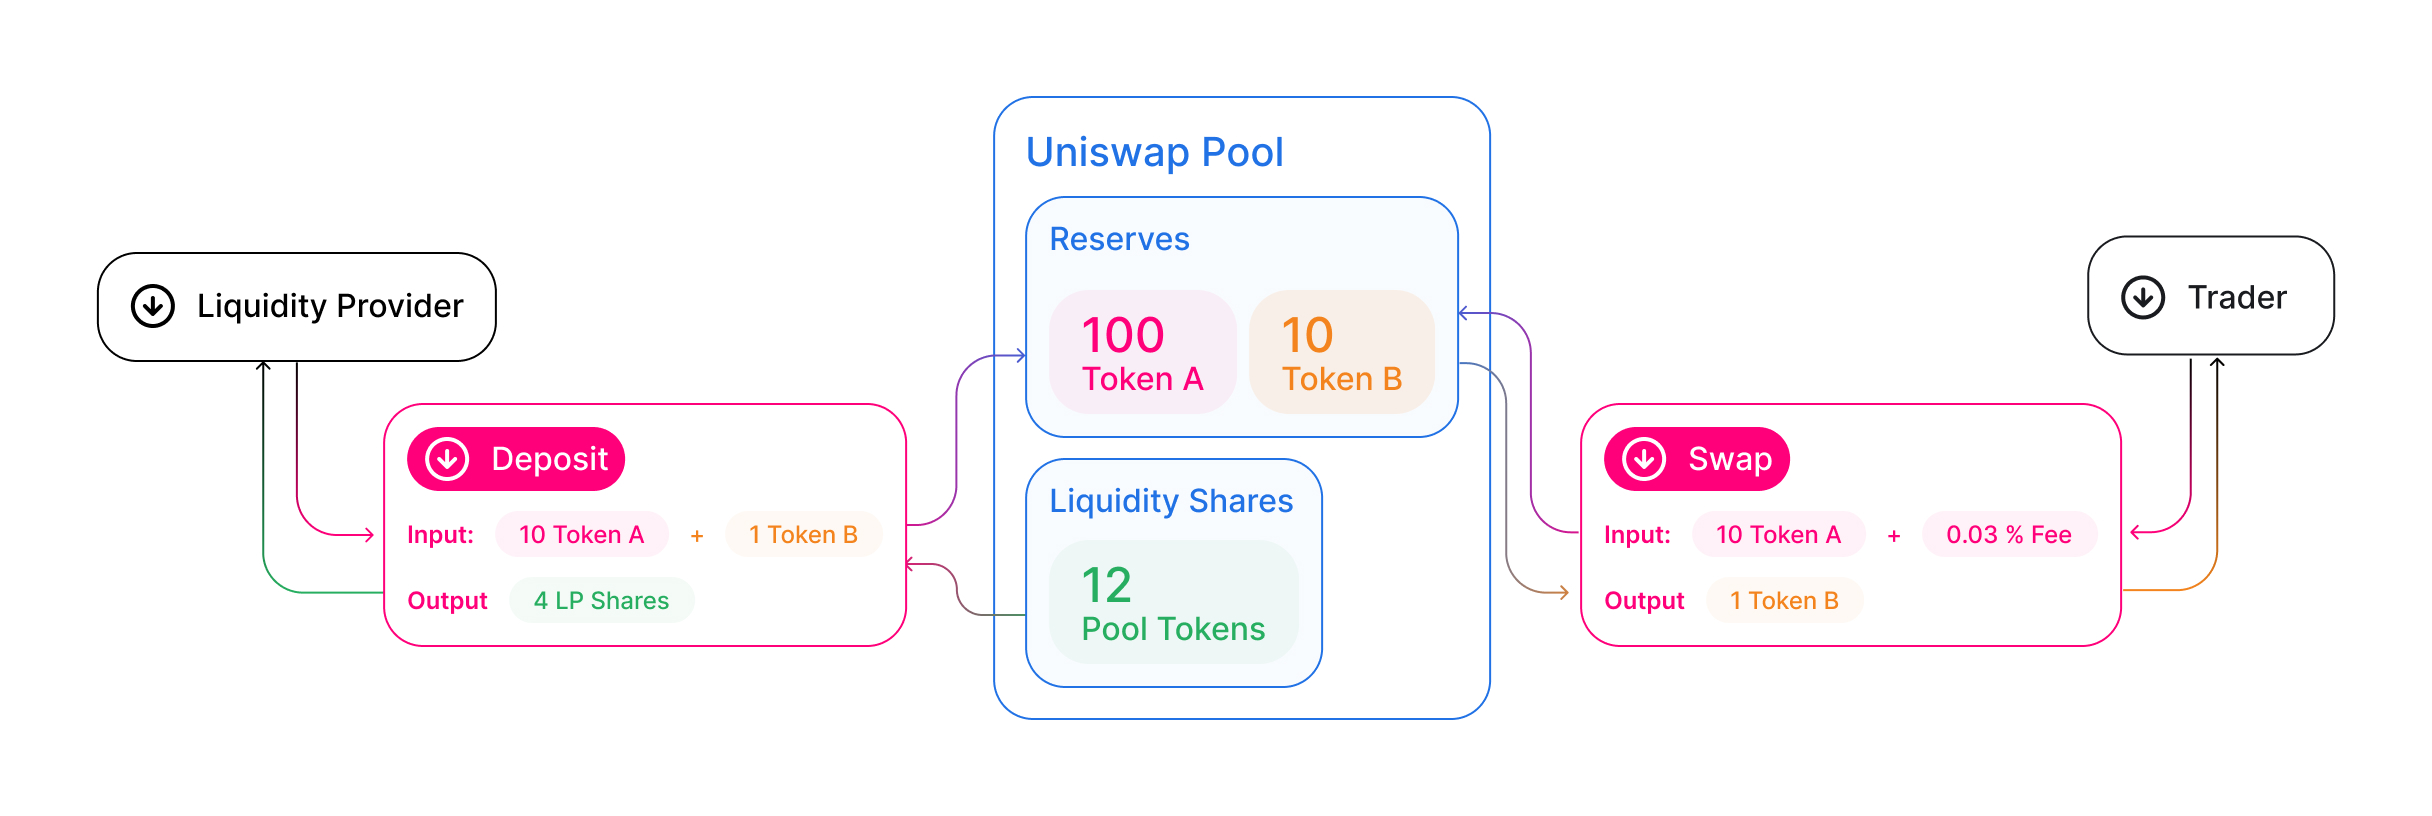
\includegraphics[width=\linewidth]{figures/uniswap-pool.jpg}
  \caption{Interactions between Uniswap liquidity providers and traders around liquidity pools (Figure retrieved from \cite{HowUniswapWorks})}
  \label{fig:uniswap}
\end{figure}

To determine the swapping price, every liquidity pool preserves the \textit{constant product} formula: $reserve_A * reserve_B = k$, where $k$ is a preserved constant \cite{HowUniswapWorks} to ensure that from the reference frame of a swap, when certain amount of one token is withdrawn, effectively reducing the reserve of that token, then an appropriate amount of the other token must be deposited in return to maintain the constant $k$. It is important to note that this formula only applies to swap of tokens, the provisioning of liquidity from LPs can, however, change the constant $k$ over time. Even though, the price of tokens in Uniswap pools can be affected by liquidity provisioning and trading, the pool price will eventually converge to the market-clearing price due to arbitrage opportunities when there is a large deviation between Uniswap price and true market price, e.g. on CEXs \cite{Adams2020UniswapVC}. 


For a concrete example case, if Alice deposits 1000 ETH and 100,000 DAI into an empty WETH/DAI pool, then, the swapping rate of the pool will be 1 ETH for 100 DAI or reversely, 1 DAI for 0.01 ETH. In addition, as DAI is a stable coin at the price of \$1 for 1 DAI, the overall liquidity of the WETH/DAI pool is thus worth \$200,000. Note that since ETH is a native cryptocurrency of Ethereum and thus, not an ERC20 token, Uniswap provides a ERC20-compliant representative contract for ETH called Wrapped ETH (WETH) that allows 1:1 exchanges from ETH to WETH and vice versa to support the direct swapping at from ETH to another ERC20 token. Now, if Bob, a trader who needs 10,000 DAI but he only owns ETH, then he can use the pool to swap 100 ETH for that much DAI and additionally pays 0.3\% of 100 ETH, which equals 0.3 ETH, as swapping fees into the pool. As such, the pool reserves after the trade by Bob are 1100.3 ETH and 90,000 DAI and the new price for subsequent swaps can then be calculated according to the constant product formula described above. From Alice's side, she has earned the entire 0.3 ETH as profit since she owns 100\% DAI liquidity of the pool and this profit will be paid out to her when she redeems her deposits from the pool. 

Overall, the core of Uniswap lies in liquidity pools, which are smart contracts acting as automated market makers as well as trading venue for the tradable token pair they represent. With the fee mechanism in place, Uniswap incentivizes the open market participants to become LPs and thereby, facilitating more and more trades on the market, while traders can instantly receive the tokens to meet their demands through token swapping. 